\documentclass[11pt,a4paper]{article}
\usepackage[margin=2.5cm]{geometry}
\usepackage[T1]{fontenc}
\usepackage[utf8]{inputenc}
\usepackage{lmodern,textcomp,amsmath,amssymb}
\usepackage{graphicx}
\usepackage{setspace}
\usepackage{titlesec}
\usepackage[hidelinks]{hyperref}
\setstretch{1.15}
\setlength{\parindent}{0pt}
\setlength{\parskip}{0.6em}
\titleformat{\section}{\Large\bfseries}{}{0pt}{}
\titleformat{\subsection}{\large\bfseries}{}{0pt}{}
\titleformat{\subsubsection}{\normalsize\bfseries}{}{0pt}{}
\begin{document}

\section*{Intermittent working-memory through NMDA-sustained persistent activity}

\begin{center}Joao Barbosa\end{center}

\begin{center}Cognitive Neuroimaging Unit, INSERM, CEA, CNRS, Université Paris-Saclay, NeuroSpin center \& Institut de neuromodulation, GHU Paris, psychiatrie et neurosciences, centre hospitalier Sainte-Anne, pôle hospitalo-universitaire 15, Université Paris Cité, Paris, France.\end{center}

\section*{Abstract}

Working memory is classically attributed to persistent spiking sustained by slow NMDA receptor (NMDAr) currents. This view has been challenged by large-scale prefrontal recordings in which the remembered item is decoded only intermittently on single trials, suggesting that memories survive silent periods through synaptic facilitation. Here we show that intermittent coding emerges from canonical attractor networks with fixed synapses and a fluctuating, attention-like global input. Brief drops in attention silence the network, but we show that NMDAr currents can bridge each silence. Fitted to monkey prefrontal cortex (PFC) recordings, a rate model reproduces the number and duration of silent states and shows that the statistics of these silent states depend on which neurons are decoded. In PFC, silent states were more frequent when the decoder used smaller or less informative subsets of neurons, suggesting that decoding-based measures of silent states might overestimate how often memory leaves spiking activity. Unlike synaptic facilitation, the NMDAr trace predicts memory loss when silences outlast a few hundred milliseconds. In line with this, monkeys made more errors the longer the memory spent in silent states, and their performance pointed to a trace of \textasciitilde{}120 ms, matching NMDAr kinetics rather than the long time scale of facilitation. Finally, we replicate the main findings in a biophysical ring-attractor network of spiking neurons with NMDAr-mediated recurrent excitation, demonstrating intermittent rate coding through persistent activity bridged by NMDAr currents.

\section*{Introduction}

Two main mechanisms have been proposed to hold information in working memory. In persistent-activity models, recurrent excitation keeps a cue-selective population firing through the delay, and slow NMDA receptor (NMDAr) currents make this activity stable (Amit and Brunel, 1997; Wang, 1999, 2001; Compte et al., 2000). Consistent with these models, blocking NMDAr markedly reduces persistent neural firing in monkey prefrontal cortex (Wang et al., 2013). In activity-silent models, the memory is instead stored in short-term synaptic facilitation and does not require ongoing spiking during maintenance (Mongillo et al., 2008; Stokes, 2015; Lundqvist et al., 2016; Miller et al., 2018; Panichello et al., 2024), and hidden memories can be reactivated after periods without decodable activity (Rose et al., 2016; Wolff et al., 2017; Barbosa et al., 2020). Notably, the two accounts rely on traces with very different time scales. NMDAr currents decay on a time scale of hundreds of milliseconds, both in cortical recordings (Vicini et al., 1998; Wang et al., 2008) and in models of persistent activity (Wang, 1999; Compte et al., 2000). On the other hand, facilitation at excitatory synapses in prefrontal cortex decays on a time scale of the order of a second, both in recordings (Thomson, 1997; Markram et al., 1998; Hempel et al., 2000; Wang et al., 2006) and in activity-silent models (Mongillo et al., 2008). Synaptic augmentation, which lasts tens of seconds, has been proposed to bridge even longer silences (Mongillo and Tsodyks, 2025).

Rigorously testing predictions of these models requires single-trial resolution (Lundqvist et al., 2018), which only recently became possible with the advance of large-scale, intracranial recordings (Williams and Linderman, 2021; Urai et al., 2022). Recent studies leveraging these techniques show that working-memory information in prefrontal cortex (PFC) fluctuates within a trial (Panichello et al., 2024; Tao and Libedinsky, 2024; Mozumder et al., 2026). Panichello et al. (2024) found that decoding alternates between \textit{On states} (when the memory can be decoded) and \textit{Off states} (when it cannot) and concluded that synaptic changes carry the memory through \textit{Off states}. Tao and Libedinsky (2024) found rare periods of 43–414 ms in which all simultaneously recorded selective neurons were silent for longer than expected by chance, and concluded that short-term plasticity is needed in a small fraction of trials. Finally, Mozumder et al. (2026) found that persistent activity is asynchronous across neurons, with no population silences beyond chance. In their recordings, decoding \textit{Off states} came with reduced but not abolished tuning and were synchronized between prefrontal and parietal cortex. The authors interpreted this cross-region synchronization as evidence for global fluctuations driving \textit{Off states}.

Here, we ask whether a single persistent-activity mechanism can account for these observations and propose that intermittent decoding does not require short-term plasticity and is in fact more consistent with the NMDAr account. To illustrate this, we modelled working memory with a classic attractor model, in which two cue-selective populations sustain their firing through recurrent excitation mediated by slow NMDAr currents and compete through shared inhibition (Wang, 2002; Wong and Wang, 2006). The synchrony of \textit{Off states} seen across prefrontal and parietal cortex (Mozumder et al., 2026) points to a common input as their source. Further, attention, which waxes and wanes on sub-second time scales (Fiebelkorn and Kastner, 2019), is a natural candidate for such common input. We therefore added to the model a fluctuating attentional input common to both populations, whose brief drops silence both populations. During each silence, slow NMDAr currents carry the memory across, so the cued population resumes firing when the attentional signal returns. We read out the model with the same decoding and \textit{On/Off} criteria as Panichello et al. (2024) and fit how often, for how long and how deeply attention lapses to the \textit{On/Off} statistics of these recordings. The model quantitatively reproduces the number and length of \textit{On and Off states} while keeping the memory in persistent activity. Our reanalyses of the PFC recordings showed that \textit{Off states} are more frequent when fewer (or less selective) neurons are decoded, so their frequency partly reflects how well the recorded sample reads out the memory, and the attractor model predicts this dependence for decoded populations it was never fitted to. Unlike a model in which short-term facilitation carries the memory, the NMDAr model predicts that errors grow with the time spent \textit{Off}, as we found in the recordings. Fitted to the monkeys' performance, the decline in accuracy with \textit{Off} time points to a trace of about 120 ms, which matches NMDAr kinetics rather than facilitation. Finally, we show that a classic biophysical ring-attractor network of spiking neurons (Compte et al., 2000) with an added fluctuating global input is enough to reproduce the main results of Panichello et al. (2024) without short-term plasticity. Finally, the spiking network predicted that spiking activity during \textit{Off }states carry stimulus information, which we confirm in PFC recordings. Previous work took intermittent decoding as evidence that persistent activity is not sufficient for working memory, our results show that this evidence has a more likely explanation within the standard persistent-activity account.

\section*{Results}

\subsection*{Input dips produce \textit{Off states} and NMDAr carries the memory across them}

We started by modelling \textit{On/Off} states using a variation of the classic two-pool attractor model (Wang, 2002; Wong and Wang, 2006), with two memory pools that excite themselves through NMDAr currents and compete through shared inhibition (Methods). We extended this classic model with an input common to both pools that fluctuates, which we interpret as an attentional signal, since attention is known to wax and wane on sub-second time scales (see Discussion). Without fluctuations in its input, a cued pool stays active after the cue offset and cue decoding is strong (Fig. 1a, first second after the cue). With brief dips in this input, both pools fall silent and decoding drops to chance (Fig. 1a, after 1,000 ms). During each dip, the NMDAr gating of the cued pool decays with a time constant of 150 ms and stays higher than that of the uncued pool. When the input returns, the pool with more NMDAr gating wins the competition. These periods of low firing and chance decoding therefore do not erase the memory, because NMDAr gating carries it across each silence and the cue is still correctly remembered at the end of the delay.

To compare the model with the data, we read it out like the recordings (Supplementary Fig. 1; Methods). In the recordings, Panichello et al. (2024) trained a decoder on the neurons of each session and expressed on every 100 ms how well it read out the cue as a z score relative to a null distribution obtained by shuffling the cue labels. Since the model has no neurons, we built the equivalent score from its two pools. The evidence for the cue is the difference between the cued and uncued pool rates (\ensuremath{\Delta}r) in the same 100 ms windows. We converted this difference into z units by multiplying it by a gain \textit{c} and adding read-out noise \textit{\ensuremath{\eta}}, whose variance and temporal correlations were estimated from PFC recordings using the decoder output before the cue (Methods). Simulations with synthetic neurons validate this read-out (Supplementary Fig. 1e–i). \textit{On and Off states} (red and cyan in Fig. 1a) are then labelled with similar thresholds of Panichello et al. (2024) (dashed lines in Fig. 1a). Read out this way, the model alternates between \textit{On and Off states} (Fig. 1a, bottom, mid gain). Both length distributions peak near 100 ms and have long tails (Fig. 1b), qualitatively like those in PFC recordings (Panichello et al., 2024). Because the dips act on the whole network, the model also predicts that \textit{Off} states occur simultaneously in different groups of neurons. To test this, we split the units of each recorded session at random into two halves and decoded the cue from each half separately. The z scores of the two halves were correlated within trials during the delay (r = 0.31 \ensuremath{\pm} 0.03, mean \ensuremath{\pm} s.e.m. over 25 sessions; p = 1\ensuremath{\times}10\textsuperscript{\ensuremath{-}}\textsuperscript{1}\textsuperscript{0}, t-test against zero), as expected from a common input. Importantly, we found that \textit{On/Off} statistics depend strongly on the read-out gain, which in our model reflects how informative the decoded neurons are about the cue. Keeping the dynamics and noise fixed for this particular simulated trial and halving the gain (as for a less informative sample of neuron) gave more \textit{Off} states and far fewer \textit{On} states, whereas doubling it (as for a more informative sample) gave fewer and shorter \textit{Off states} and more \textit{On states} (Fig. 1a, bottom, low and high gain, and Fig. 1b for many trials). This predicts that \textit{On}/\textit{Off} statistics measured in the recordings depend on how informative the decoded neurons are. In the next sections, we test this prediction and ask whether the model matches the data quantitatively.

\begin{center}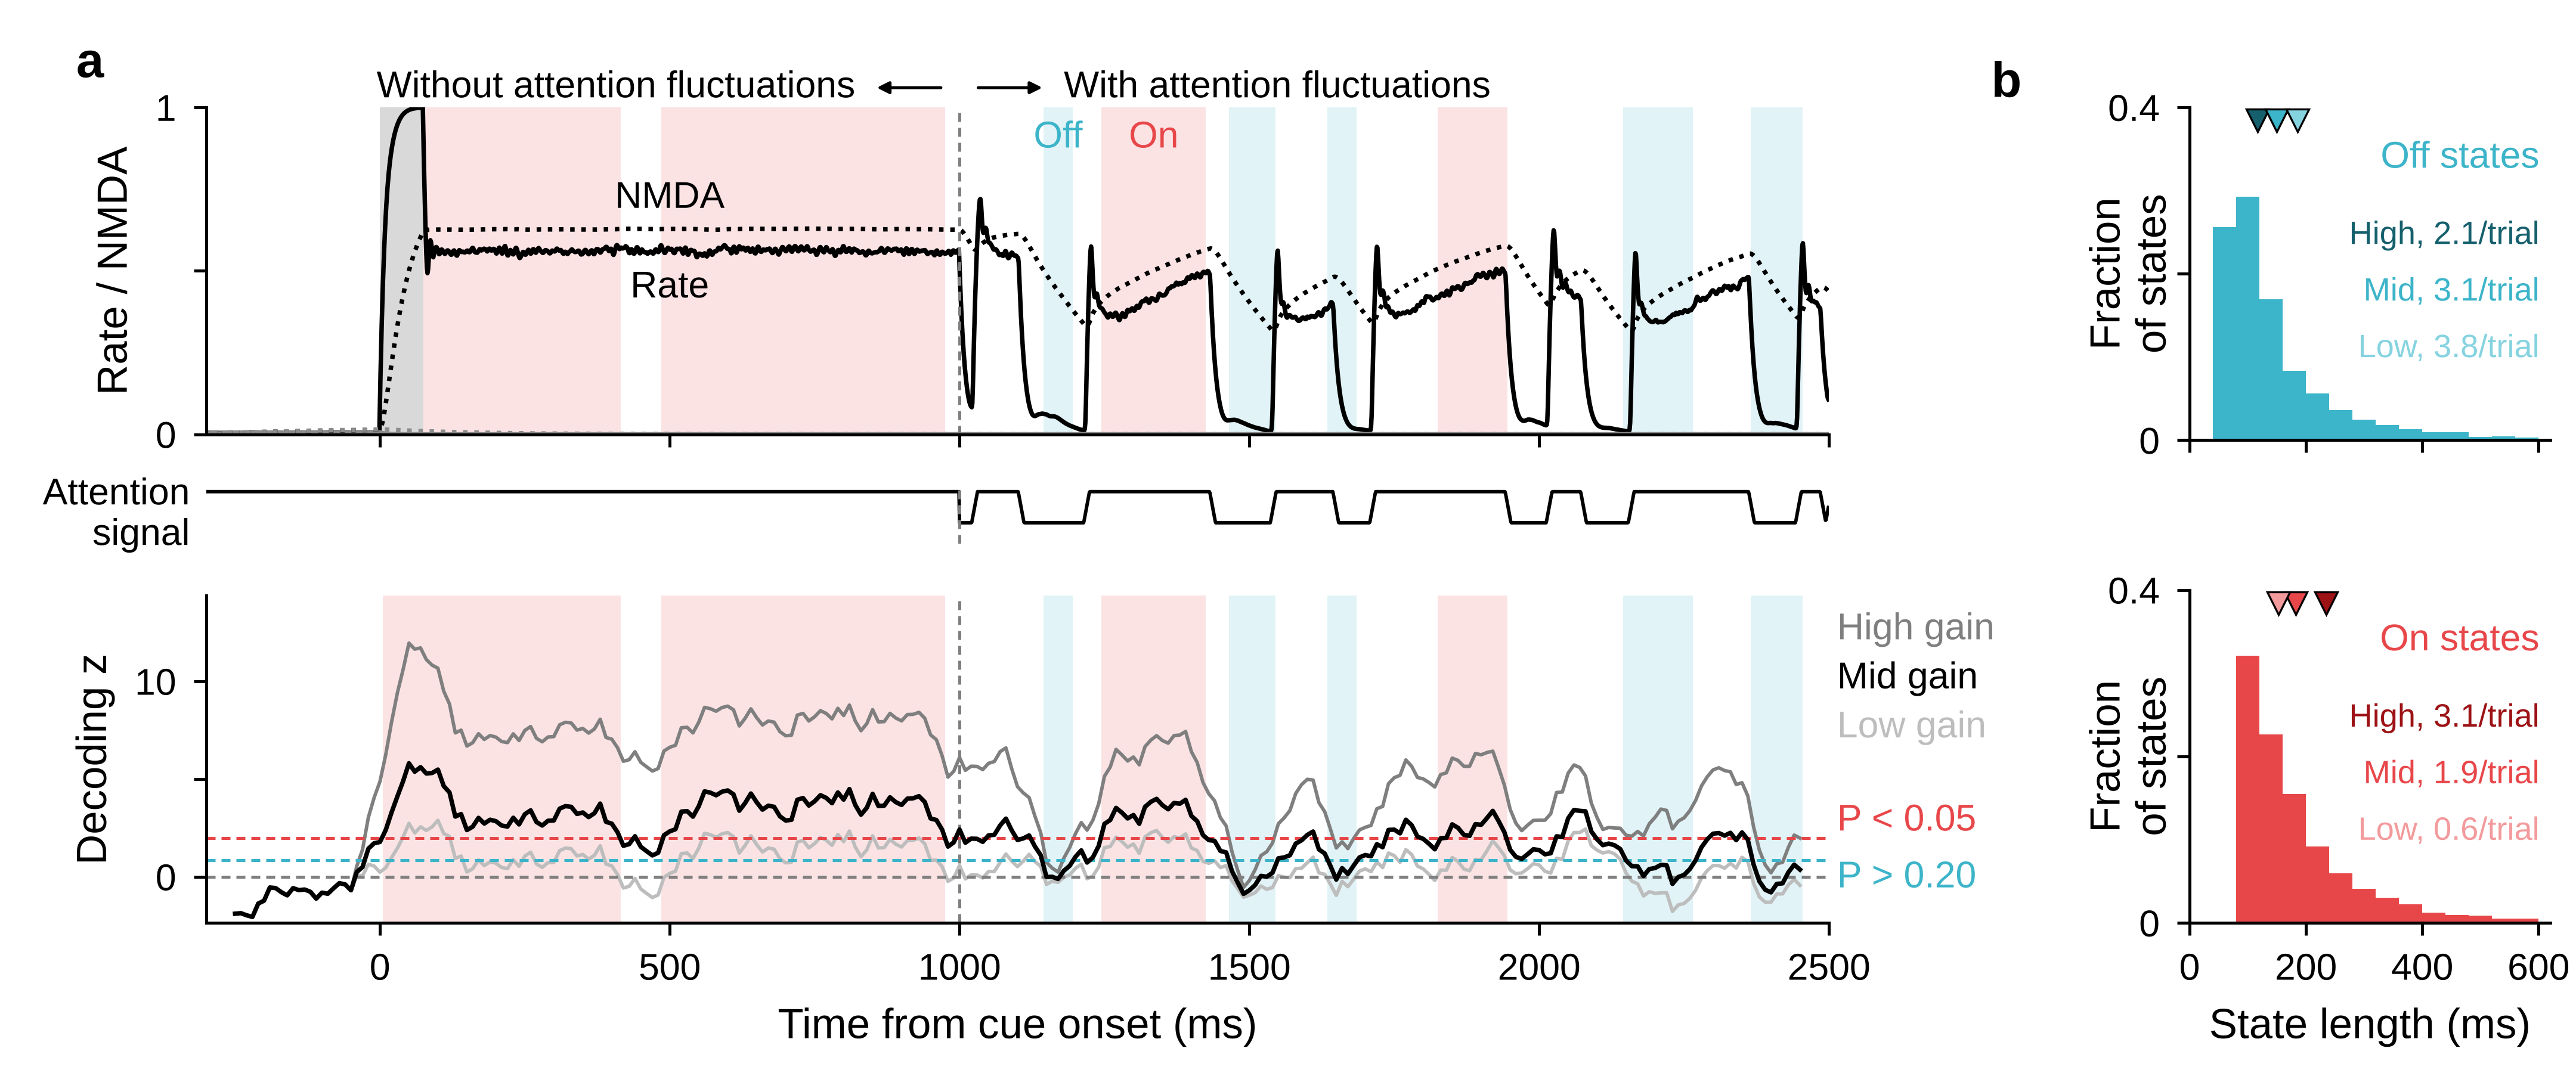
\includegraphics[width=1.000\textwidth]{figures/fig01.png}\end{center}

\textbf{Figure 1. Input dips create }\textbf{\textit{On and Off states}}\textbf{, and NMDAr carries the memory. }a, Example trial. Top: rates of the cued (black) and uncued (grey) pools, relative to the maximum rate, and their NMDAr gating (dotted); grey shading marks the cue. Middle: common input (attention signal), constant for the first 1,000 ms after the cue and with dips afterwards. The dip-free first second is shown for illustration only; in all other simulated trials, dips occur throughout the delay. Bottom: decoding z score of the same trial read out with the calibrated gain \textit{c} (mid gain, black), twice this gain (high gain, dark grey) and half of it (low gain, light grey), with the same read-out noise. \textit{On} (red) and \textit{Off} (cyan) states are those of the mid-gain read-out. Dashed lines: \textit{On} threshold (z = 1.96) and \textit{Off} threshold (z = 0.84), as in Panichello et al. (2024). b, Length distributions of \textit{Off} (top) and \textit{On} (bottom) states in the model at the mid gain, as fractions of states in 40 ms bins (2,000 simulated trials). Triangles: mean state length at the three gains (dark, high; medium, mid; light, low), with the mean number of states per trial.

\subsection*{\textit{On/Off} statistics depend on which neurons are decoded}

In our reanalysis of the PFC recordings of Panichello et al. (2024), we found that \textit{On/Off} statistics depend strongly on how informative the decoded neurons are (Fig. 2; Supplementary Fig. 2). Decoders using the most cue-selective neurons spend much more of the delay \textit{On} (Fig. 2f; Supplementary Fig. 2f), and less \textit{Off} (Fig. 2c; Supplementary Fig. 2c), than decoders using the same numbers of randomly chosen neurons, which also show more \textit{Off states} per trial (paired Wilcoxon signed-rank tests over 25 sessions, p < 10\textsuperscript{\ensuremath{-}}\textsuperscript{6} for each of 5, 20 and 50 neurons; Fig. 2a; Supplementary Fig. 2a). How often a memory appears \textit{Off} therefore depends partly on how well the recorded neurons read it out. A decoder trained on a limited sample of neurons can fall to chance while the memory is still present in the activity of other, potentially unrecorded neurons. The measured fraction of time \textit{Off} is therefore an upper bound on how often the memory leaves spiking activity. We then asked if our model could explain this dependence.

\begin{center}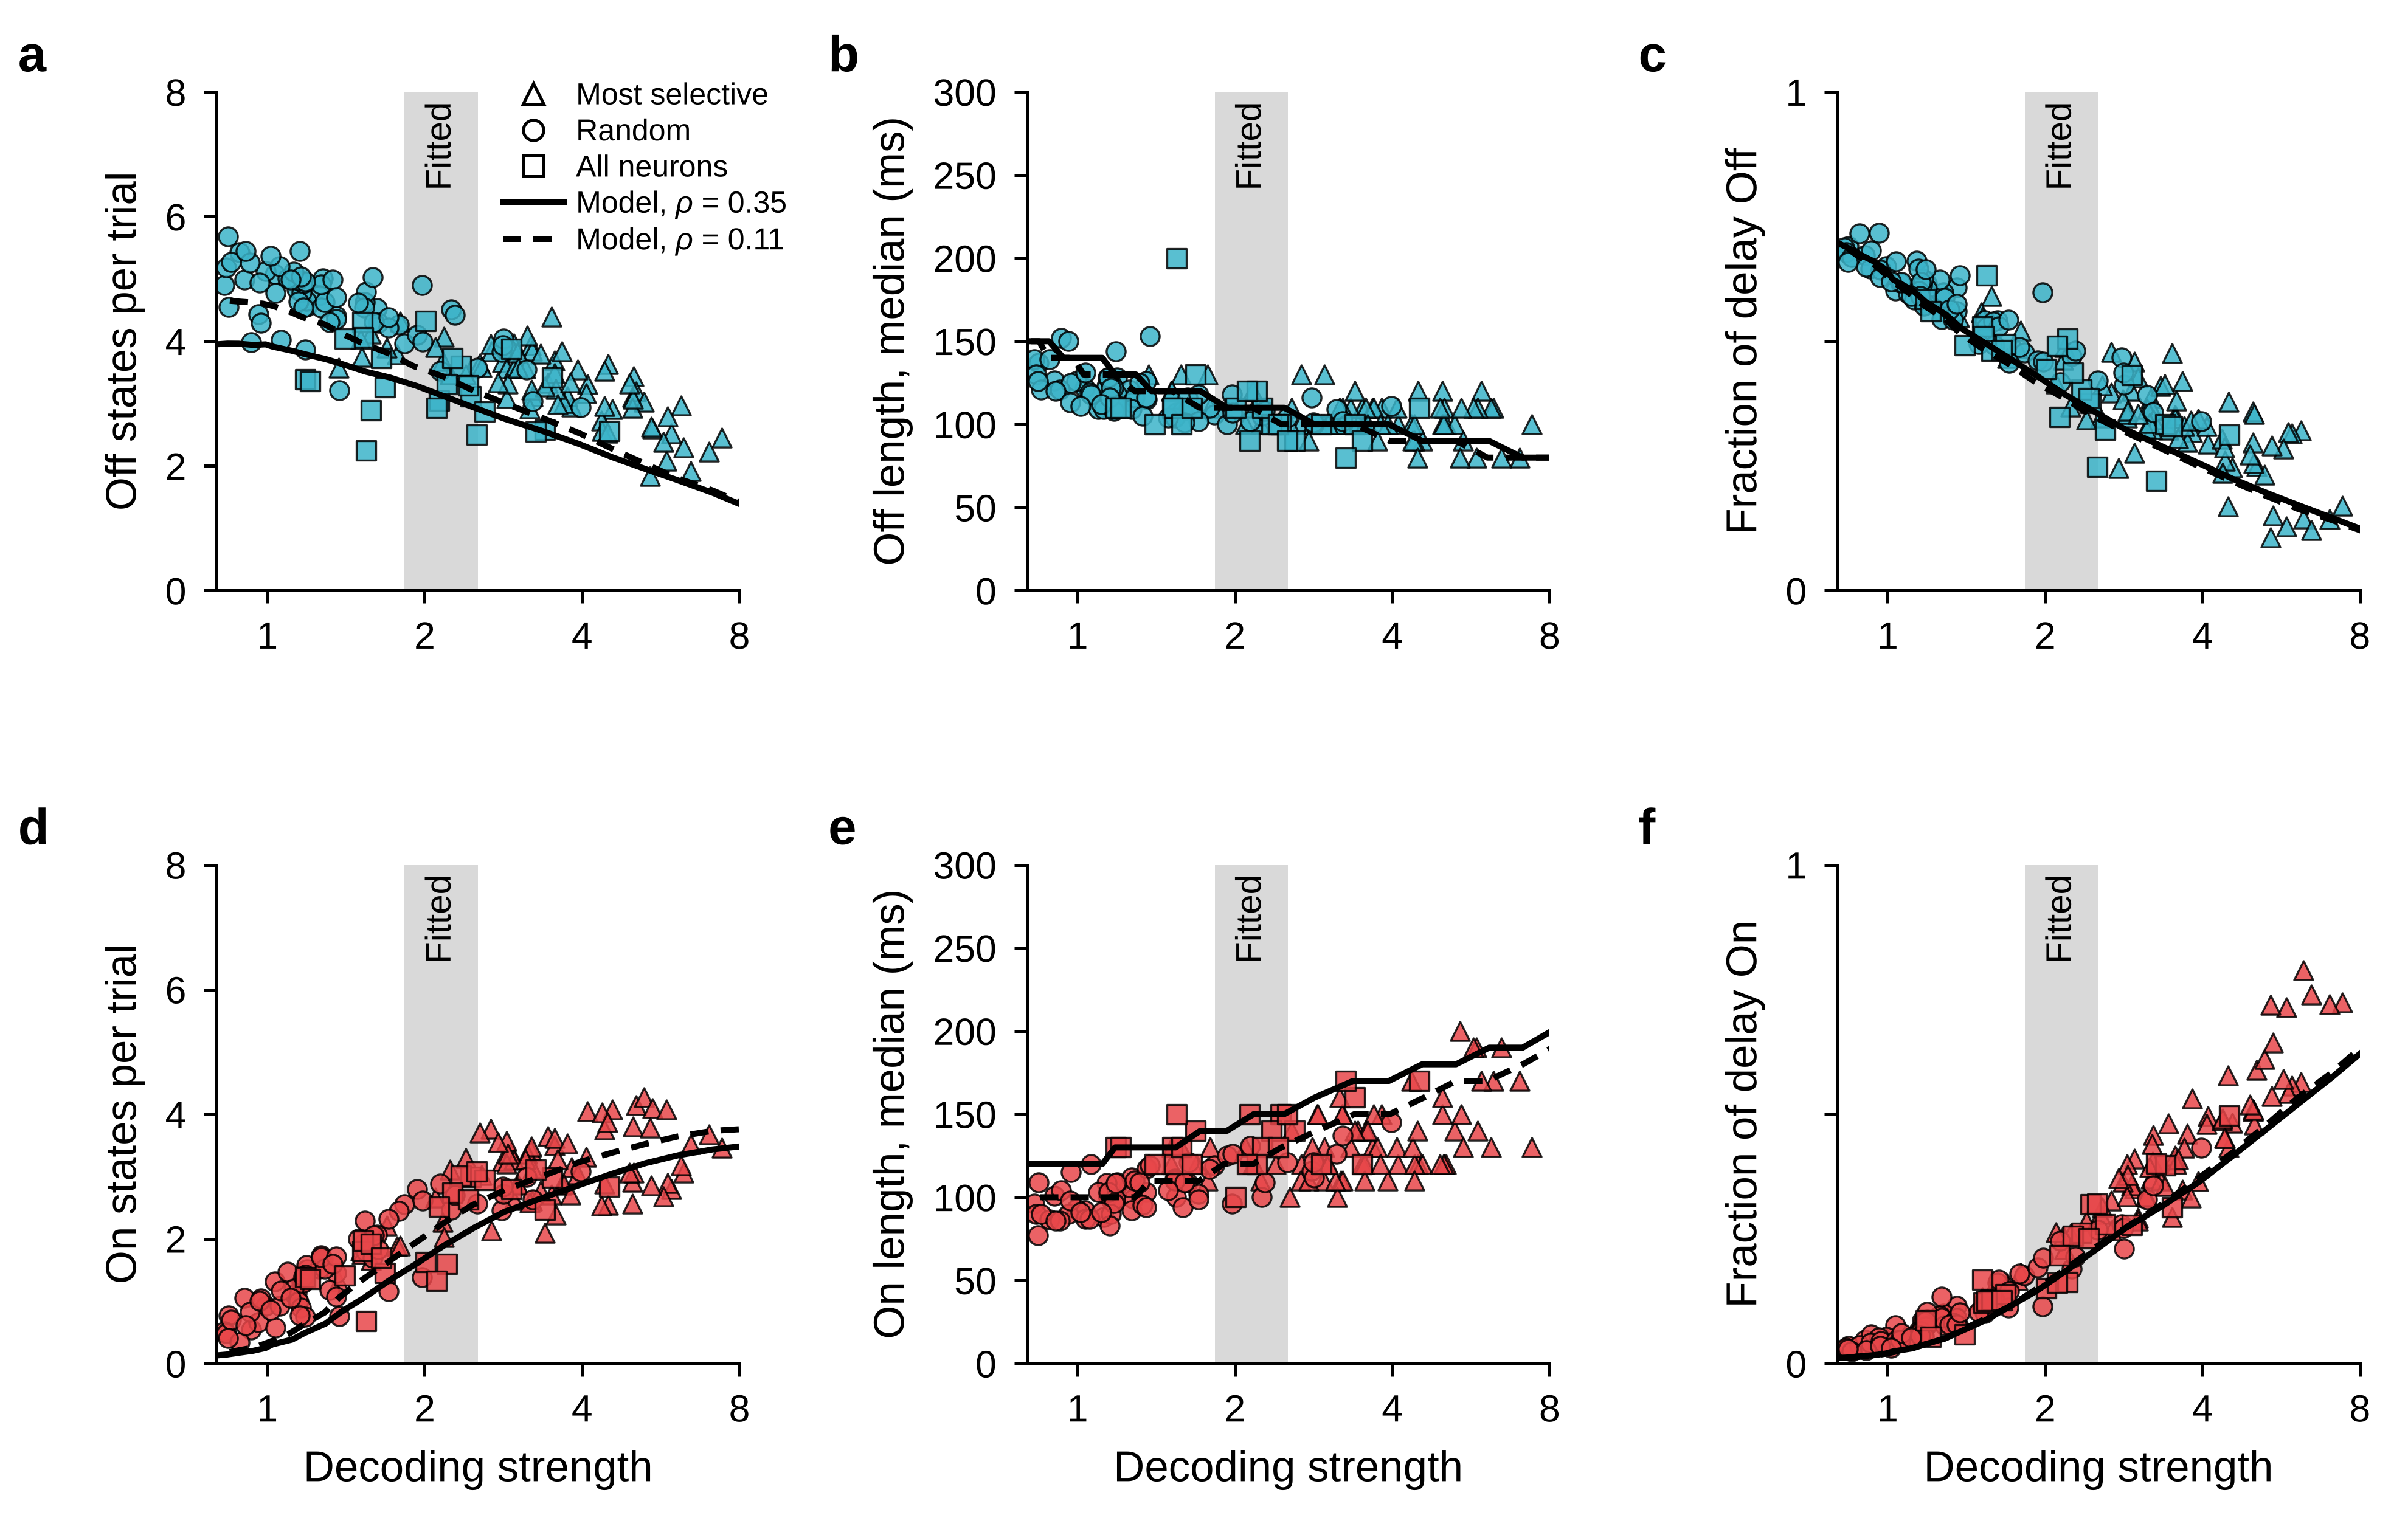
\includegraphics[width=0.923\textwidth]{figures/fig02.png}\end{center}

\textbf{Figure 2. The model predicts how }\textbf{\textit{On/Off}}\textbf{ statistics change with the decoded population. }\textit{On/Off} statistics against decoding strength (Methods). Each symbol is one session read out with one decoded population: the 5, 20 or 50 most cue-selective neurons (triangles), the same numbers of random neurons (circles) or all neurons (squares). a–c, \textit{Off} states per trial, median \textit{Off} length and fraction of the delay \textit{Off} (cyan). d–f, the same for \textit{On} states (red). Lines: the model, fitted to all neurons only (grey band: their decoding strength, mean \ensuremath{\pm} 2 SEM over 25 sessions) and read out at varying gain without refitting, with the read-out noise of all neurons (solid, \ensuremath{\rho} = 0.35) or of the smaller populations (dashed, \ensuremath{\rho} = 0.11; Methods).

To test this, we fitted the model dynamics to the decoder using all neurons in 25 sessions (Methods). The model matches the data well in \textit{Off states} per trial (3.1 vs 3.3), \textit{Off} median length (110 vs 112 ms), \textit{On states} per trial (1.9 vs 2.1) and \textit{On} median length (140 vs 134 ms) (Fig. 2, grey band; Supplementary Fig. 2). We then kept the dynamics fixed and, for each of the six other decoded populations, changed only the read-out without refitting any parameters. Its gain was calibrated on that population's decoding strength and its noise on that population's pre-cue z (Methods). The model therefore predicts the shift between selective and random neurons (Fig. 2; Supplementary Figs. 2 and 3).

\subsection*{Errors increase with time \textit{Off}, as expected from an NMDAr trace}

Panichello et al. (2024), like our analyses so far, used correct trials only. However, we found that error trials help distinguish between the two accounts of working memory. NMDAr currents and short-term synaptic facilitation can both carry a memory across brief \textit{Off states}, but on very different time scales. In our model, NMDAr gating decays with a time constant of 150 ms, whereas facilitation decays on a time scale of the order of a second (Wang et al., 2006; Mongillo et al., 2008), comparable to the length of the whole memory period. To see explicitly what each mechanism predicts regarding error trials, we compared our model with a version in which facilitation replaces NMDAr gating (STP model; Methods). Fitted in the same way, it reproduced the \textit{On/Off} statistics about as well as the NMDAr model (Supplementary Fig. 4). This is expected, because in both models \textit{Off states }are driven by lapses of attention, which facilitation (\ensuremath{\tau}\textsubscript{f} = 1.5 s) bridges even more easily than NMDAr gating (\ensuremath{\tau}N = 150 ms). We then silenced each model with a single dip in the common input of increasing duration (Methods). The NMDAr model held the memory for silences of up to 350 ms and lost it for every silence from 400 ms on, because the NMDAr trace had decayed too far for the cued pool to restart (about 2.5 \ensuremath{\tau}N), whereas the STP model held the memory for silences as long as 1 s (Fig. 3a). The NMDAr account therefore predicts that errors become more frequent when the memory stays \textit{Off} for long, whereas facilitation predicts no such relation for silences shorter than its own decay, which here spans the whole delay.

We tested this prediction by comparing \textit{Off} statistics between correct and error trials (Methods). We modelled errors with a single logistic mixed model of three statistics of the \textit{Off} states in the delay (total \textit{Off} time, the number of \textit{Off} states and whether the delay ended \textit{Off}) together with whether the previous trial was an error, and with cue location and monkey as covariates (Methods). Within sessions, the odds of an error increased with the total \textit{Off} time (\ensuremath{\beta} = 0.24, 95\% CI 0.15–0.33, p = 3\ensuremath{\times}10\textsuperscript{\ensuremath{-}}\textsuperscript{5}) and when the delay ended \textit{Off} (\ensuremath{\beta} = 0.22, 95\% CI 0.11–0.33, p = 7\ensuremath{\times}10\textsuperscript{\ensuremath{-}}\textsuperscript{4}), but not with the number of \textit{Off states} (p = 0.14; Fig. 3b). Errors were also more likely after an error (\ensuremath{\beta} = 0.11, 95\% CI 0.04–0.18, p = 0.02). Errors thus depended on how long the memory was \textit{Off}, not on how often it went \textit{Off.} The effect of total \textit{Off} time was clear in monkey H (\ensuremath{\beta} = 0.26, p = 0.007) and weaker in monkeys A (\ensuremath{\beta} = 0.13, p = 0.09) and J (\ensuremath{\beta} = 0.03, p = 0.85).

Finally, we asked which time constant of the trace best explains how performance falls with \textit{Off} time. We varied \ensuremath{\tau}N in the fitted NMDAr model, keeping the dip statistics and all other parameters unchanged, and simulated each version with the same random dips, read out as the data. We linked the probability that the memory was held to the probability of a correct response, assuming that the monkeys guess after a memory loss (Methods). With the best-fitting \ensuremath{\tau}N of 123 ms, the model reproduced the decline of the pooled fraction correct (Fig. 3c). Resampling sessions gave a 95\% confidence interval of 101–190 ms (Fig. 3d). The decline of performance with \textit{Off} time thus calls for a trace of about 120 ms, close to measured NMDAr kinetics and to the 150 ms assumed in the fitted model, and far shorter than the time scale of facilitation.

\begin{center}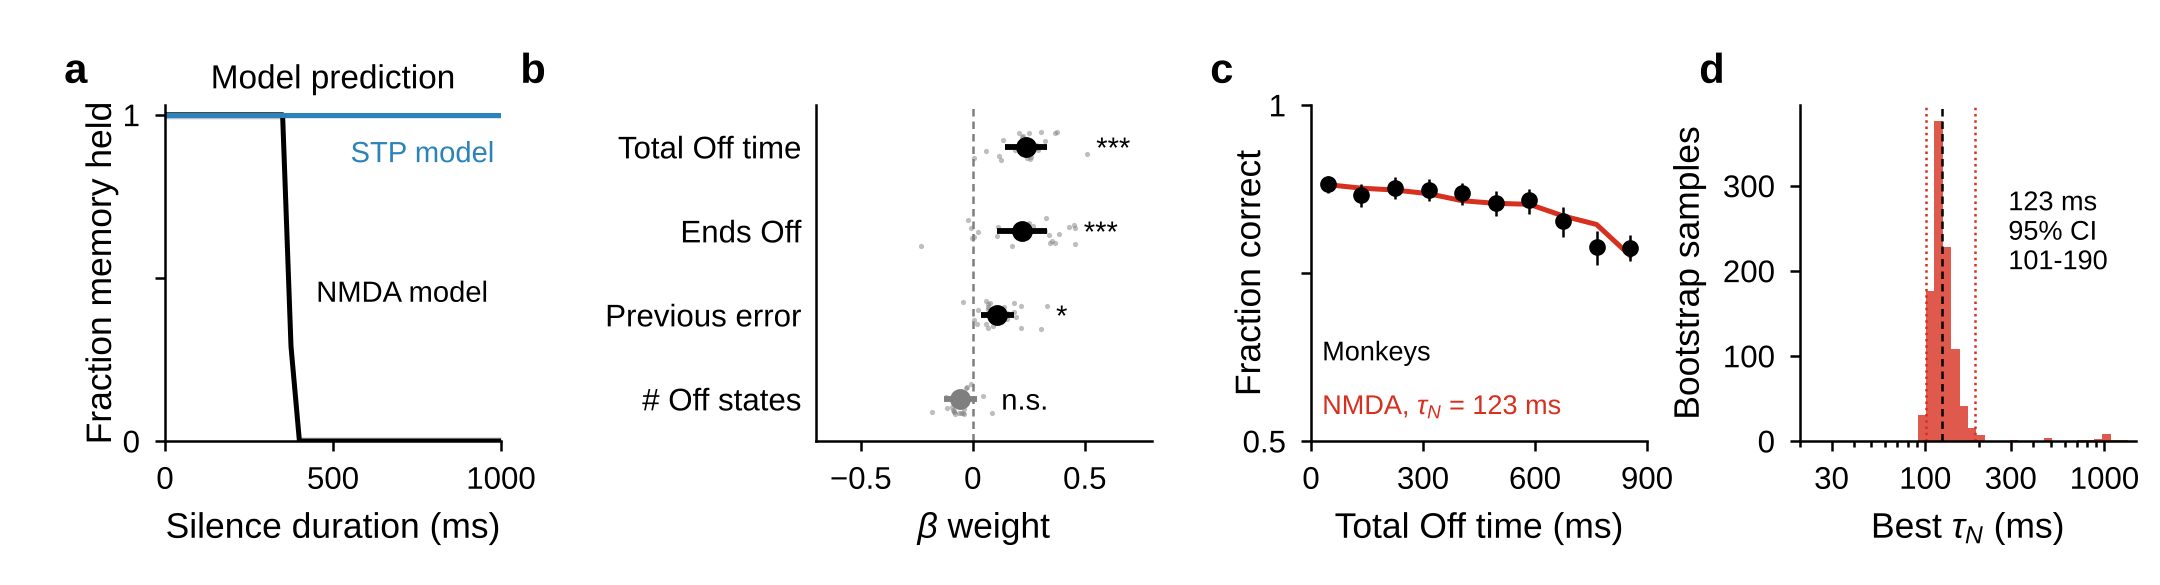
\includegraphics[width=1.000\textwidth]{figures/fig03.png}\end{center}

\textbf{Figure 3. Errors increase with time }\textbf{\textit{Off}}\textbf{, and the decline in performance points to a trace of about 120 ms.} \textbf{a}, Model prediction: fraction of trials with the memory held against the duration of a single silence, imposed by one dip of the common input (0 to 1 s in 25 ms steps, 300 trials per duration), for the NMDAr model (black) and the STP model (blue). Memory was scored on the model, without read-out (Methods). \textbf{b}, Weights (\ensuremath{\beta}) of the total \textit{Off} time, the delay ending \textit{Off}, the previous trial being an error and the number of \textit{Off} states (delay, 500–1,400 ms after cue onset), fitted together in one logistic mixed model of errors with cue location and monkey as covariates (all 25 sessions, 15,468 trials; Methods), in order of size. Circles and lines: weight and 95\% CI (black, p < 0.05; grey, not significant). Grey dots: single sessions (weight plus the session's random slope). Likelihood-ratio tests: total \textit{Off} time, p = 3\ensuremath{\times}10\textsuperscript{\ensuremath{-}}\textsuperscript{5}; delay ending \textit{Off}, p = 7\ensuremath{\times}10\textsuperscript{\ensuremath{-}}\textsuperscript{4}; previous error, p = 0.02; number of \textit{Off states}, p = 0.14. ***p < 0.001, *p < 0.05, n.s. not significant. \textbf{c}, Fraction correct against total \textit{Off} time in the delay, all 15,468 trials pooled, in 90 ms bins (black), and the NMDAr model with the best-fitting \ensuremath{\tau}N of 123 ms (red)(Methods).\textbf{ d}, Best \ensuremath{\tau}N in 1,000 bootstraps over sessions. Dashed: fit to all data. Dotted: 95\% interval (101–190 ms).

\subsection*{Intermittent rate coding in a biophysical ring-attractor network without short-term plasticity}

The rate model describes the activity of two populations, with one discrete attractor for each memory. This model leaves unclear whether its mechanism works in a continuous attractor, which can hold any location and along which the memory could drift during silences (Wimmer et al., 2014; Barbosa et al., 2020; Tschiersch et al., 2026), and in a network of spiking neurons, where NMDAr currents, recurrent inhibition and noise interact at the level of single cells. We therefore turned to the spiking network of Compte et al. (2000), a ring of 2,048 excitatory and 512 inhibitory integrate-and-fire neurons in which recurrent excitation is mediated by NMDArs and a localized bump of persistent activity holds the cued location. We used this network with minimal changes (Methods). The NMDAr decay time was set to 150 ms, as in the rate model and all excitatory neurons received the same kind of fluctuating attentional input as the rate model. In contrast to the rate model, the network was not fitted to the data. We sampled 330 of its neurons, the average number of units recorded per session in the recordings of Panichello et al. (2024), and read them out like the recordings, with the same decoder and \textit{On/Off} criteria (Methods). With a constant attentional input, the cued location was held by a stable bump of persistent activity, and decoding stayed \textit{On} throughout that period (Fig. 4a, first second after the cue). Each drop of the input silenced the bump, and decoding fell to chance. When the input returned, the bump restarted at the cued location, because the cued neurons kept more NMDAr gating through the silence than the other neurons, as in the rate model. Read out like the recordings, the network therefore alternated between \textit{On and Off states} (Fig. 4a, bottom). Both state lengths had long-tailed distributions, as in the rate model (Fig. 4b).

Finally, Panichello et al. (2024) found that neurons lose their memory tuning during \textit{Off states} and concluded that synaptic changes carry the memory through these periods. We applied their cross-validated analysis to the spiking network. Held-out neurons were strongly tuned to the cued location during \textit{On states} and barely tuned during \textit{Off states} (Fig. 4c), as in the recordings. Information about the cue might still be visible at the level of the population, where weak signals of many neurons add up. We therefore first applied PCA to the eight cue-condition means of delay activity, in the network and in the recordings. In the plane of the first two components, delay activity moved toward the centre during \textit{Off} states (Fig. 4d). We then compared the shape of the per-cue averages of activity with the ring of cue means, using a Procrustes shape similarity that ignores size (Barbosa et al., 2025; Methods). Surprisingly, \textit{Off} activity kept the shape of the ring well above chance in data and model (Fig. 4e). In other words, even when the decoder labelled the memory \textit{Off}, population activity therefore still held a detectable activity code for the cued location. \textit{Off states} defined by a decoder thus overestimate how often the memory leaves spiking activity, as the dependence of \textit{On}/\textit{Off} statistics on the decoded population also suggests (Fig. 2; Supplementary Fig. 2). Together, these results show that intermittent rate coding, including the loss of single neuron tuning in \textit{Off states}, emerges in a biophysical attractor network without short-term plasticity.

\begin{center}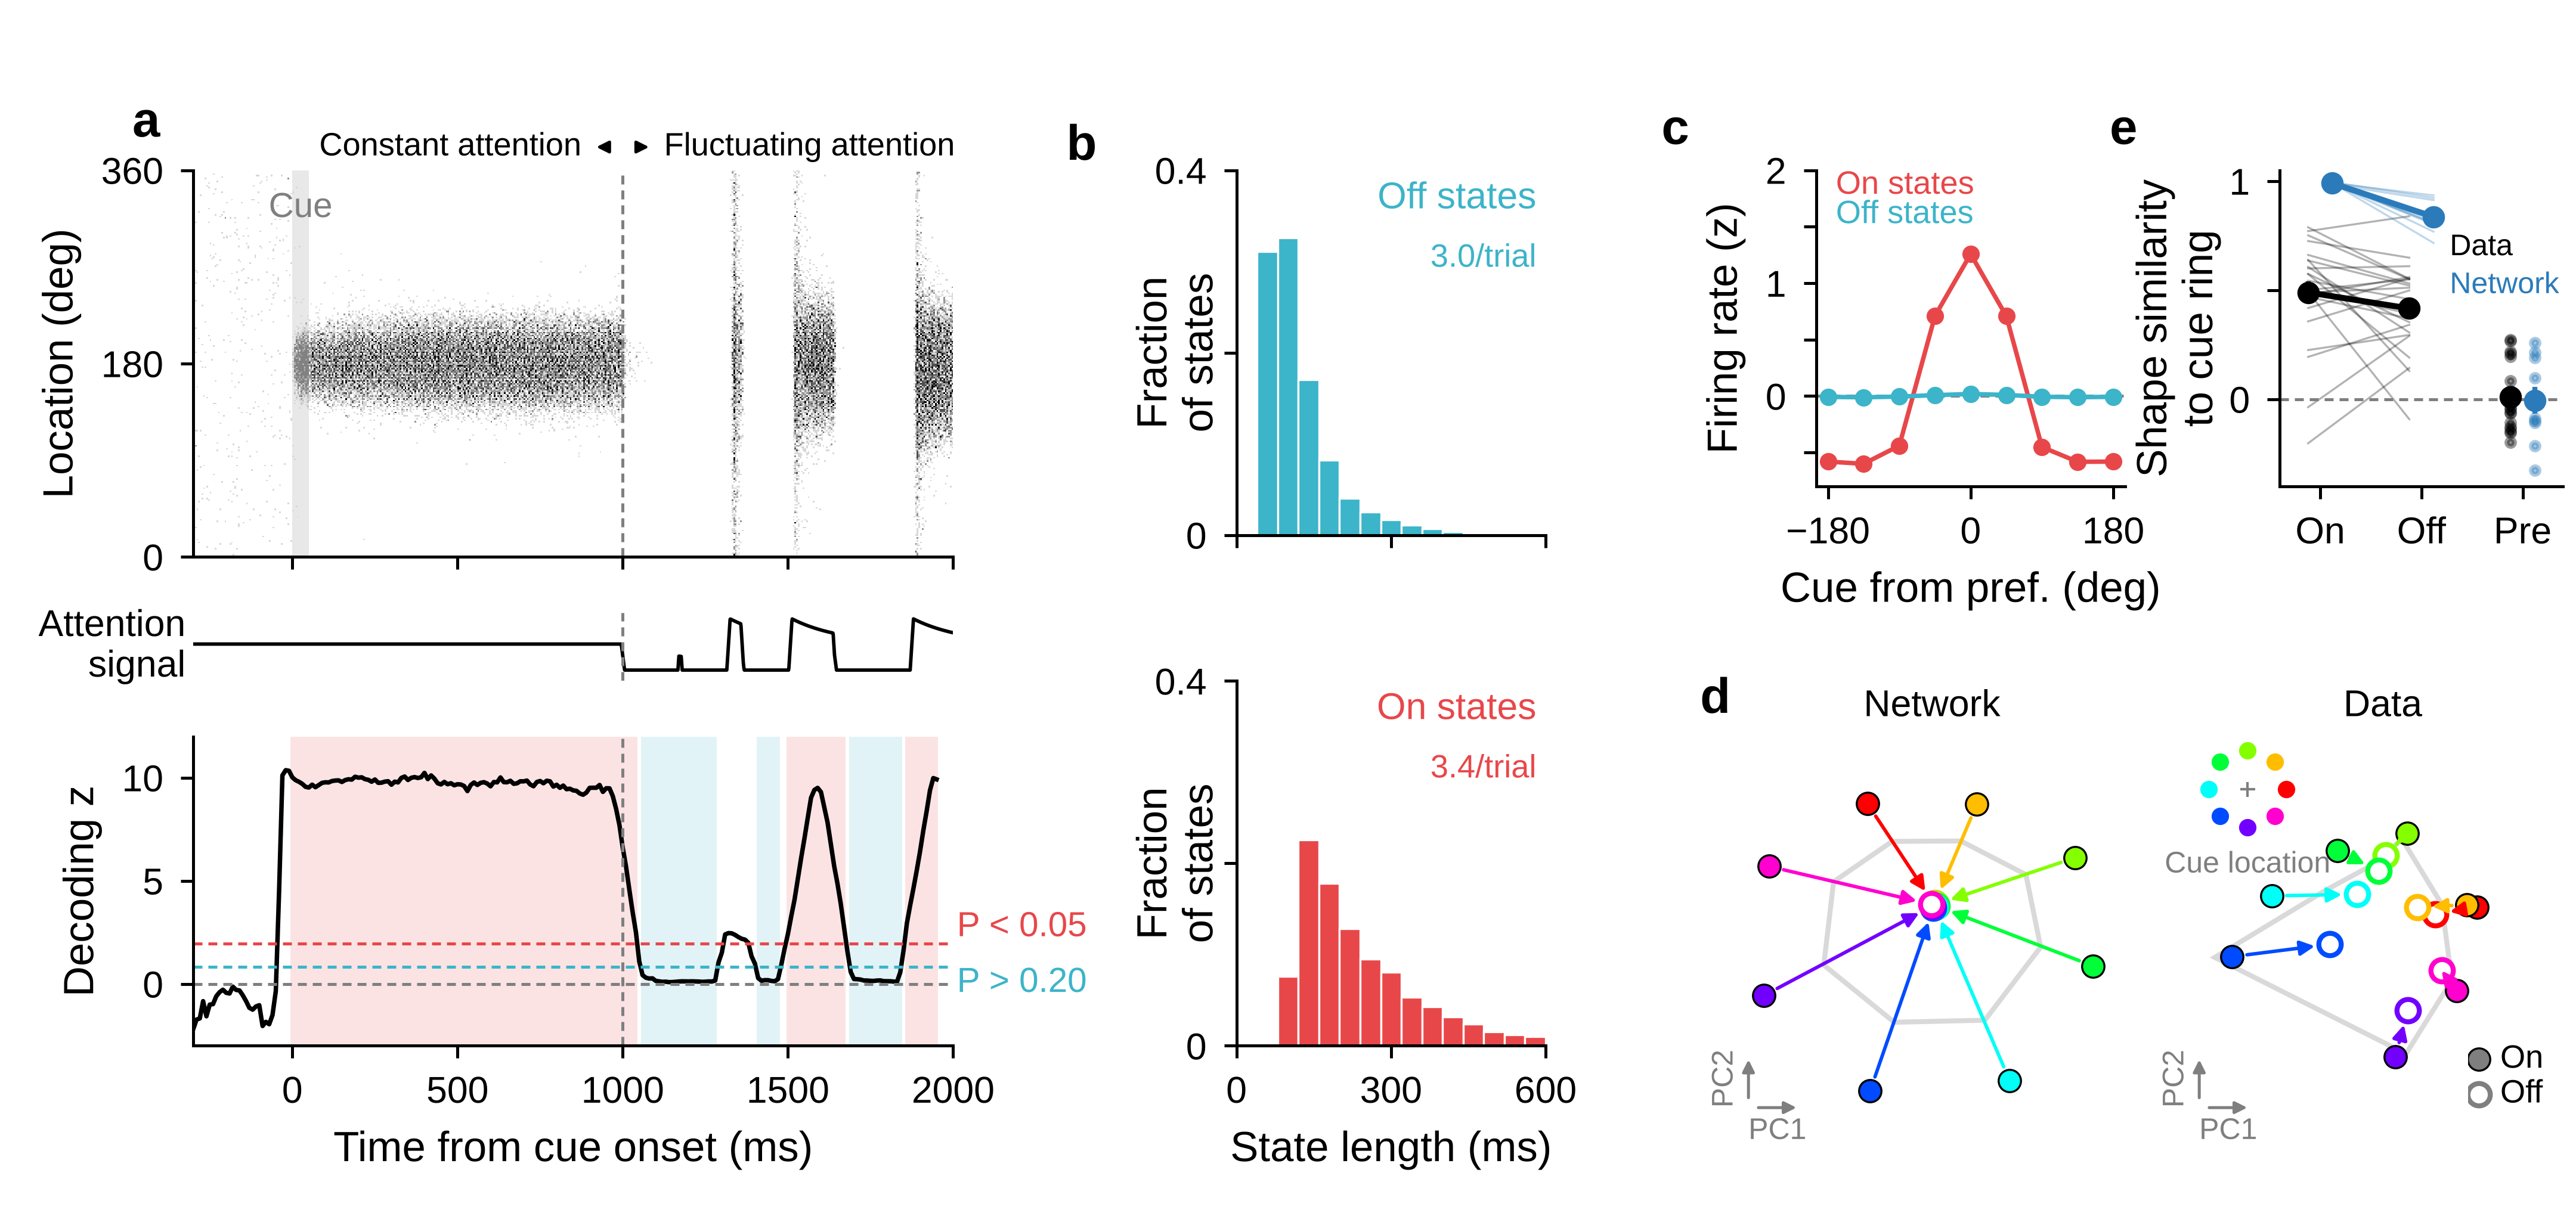
\includegraphics[width=1.000\textwidth]{figures/fig04.png}\end{center}

Figure 4. Intermittent rate coding in a spiking ring-attractor network with NMDAr currents. a, Example trial. Top: spikes of the 2,048 excitatory neurons, sorted by preferred location (counts in 5 ms and 8-neuron bins). Middle: common input (attention signal) to the excitatory neurons, constant for the first 1,000 ms after the cue and with dips afterwards, each followed by a transient overshoot. Bottom: decoding z score from 330 simulated neurons, read out like the recordings (Methods), with \textit{On} (red) and \textit{Off} (cyan) states. Dashed lines: \textit{On} threshold (z = 1.96) and \textit{Off} threshold (z = 0.84). b, Length distributions of \textit{Off} (top) and \textit{On} (bottom) states, with the mean number of states per trial (trials with the memory held in 4 simulated sessions of 480 trials). c, Cross-validated memory tuning of held-out simulated neurons during \textit{On} (red) and \textit{Off} (cyan) states, computed as in Panichello et al. (2024) (mean \ensuremath{\pm} s.e.m., 330 neurons). d, Delay activity in the plane of the first two principal components of the eight cue-condition means, for one simulated session (left) and one recorded session (221024, right). Grey, the cue-condition means. Filled and open circles, the mean position of each cue's trials during \textit{On and Off} moments, with an arrow from \textit{On} to \textit{Off}. Colours, cue location (inset). e, Shape similarity of the eight per-cue averages of activity during \textit{On} and \textit{Off} moments and before the cue (Pre) to the ring of cue means (1 \ensuremath{-} Procrustes disparity divided by the disparity with shuffled cue labels; 0, chance, dashed line). Thin lines, sessions. Thick, mean \ensuremath{\pm} s.e.m. (data, 25 sessions, black; network, 10 sessions, blue). Similarity above chance during \textit{Off} moments shows that population activity still coded the cue while decoding was \textit{Off}.

\section*{Discussion}

Recent large-scale recordings found that prefrontal decoding of a remembered item is intermittent on single trials (Panichello et al., 2024; Tao and Libedinsky, 2024; Mozumder et al., 2026), suggesting that memories survive silent periods through synaptic facilitation (Mongillo et al., 2008; Stokes, 2015; Lundqvist et al., 2016; Miller et al., 2018; Panichello et al., 2024). We showed that the same \textit{On/Off} statistics arise in conventional attractor models with fixed synapses. In the models, \textit{Off states} occur when a common input briefly drops, and the memory survives each silence because NMDAr currents decay slowly enough to bias which pool restarts. Fitted to the decoder trained on the empirical data, the rate model reproduced the number and length of \textit{On and Off states} while keeping the memory in persistent activity. Unlike a model in which short-term facilitation carries the memory, it also predicted that errors grow with the time spent \textit{Off}, which we validated in prefrontal recordings.

In the recordings, \textit{Off states} were more frequent and \textit{On states} rarer when the decoder used random rather than selective neurons. This showed that a decoder falls to chance whenever the memory signal in its sample is weak relative to its noise, not only when the memory is absent from the network. The fraction of time \textit{Off} measured from a limited sample is therefore an upper bound on how often the memory leaves spiking activity, and comparisons of \textit{Off-state} statistics across studies or brain areas need to take the decoded population into account. Population activity points the same way. In both the recordings and the spiking network, the per-cue averages of activity during \textit{Off} states kept the shape of the ring of cue means (Fig. 4e), so a decoder at chance does not mean that the cue has left population activity. The rate model captured this shift without refitting by changing only the read-out gain and noise, both calibrated from the data.

Our account is consistent with other recent recordings of \textit{Off states}. Mozumder et al. (2026) found that \textit{Off states} were synchronized between prefrontal and posterior parietal cortex, came with lower firing rates, and showed no obvious rhythmicity. A common input that reaches several areas and fluctuates irregularly, as in our fit, would produce such coordinated, aperiodic \textit{Off states}. Tao and Libedinsky (2024) likewise found that information is reduced but present between gamma bursts. Our model is compatible with both, because NMDAr currents can carry the memory across full silences but are not needed when activity is only reduced. While attention is sustained, the memory is held by persistent activity without any \textit{Off state} (Fig. 1a, first second after the cue).

We interpreted the common input as an attentional signal that is high when attention is deployed on the memorandum and drops during lapses. Two lines of evidence support this interpretation. First, Engel et al. (2016) found that spiking in macaque area V4 alternates between \textit{On and Off} episodes that occur synchronously across cortical layers. Importantly, these states were identified directly from population spiking, not from a decoder. \textit{Off} episodes lasted about 100 ms on average (102 ms during stimulus-driven and 118 ms during spontaneous activity), close to the \textit{Off states} in prefrontal decoding (about 110 ms) and within the time an NMDAr trace can bridge. Spatial attention lengthened \textit{On} episodes and made transitions less frequent, and monkeys detected a stimulus change more often when it occurred during an \textit{On} episode than during an \textit{Off} episode. Second, sustained attention samples the environment rhythmically rather than continuously. In humans, detection of threshold stimuli depends on the phase of ongoing EEG oscillations near 7 Hz (Busch et al., 2009), especially at attended locations (Busch and VanRullen, 2010), and when attention is divided between two locations, detection at each fluctuates at about 4 Hz (Landau and Fries, 2012). Similarly in monkeys, frontal eye field and lateral intraparietal activity alternates at theta frequencies (3–8 Hz) between periods of enhanced perception and periods in which attention is more likely to shift (Fiebelkorn et al., 2018), and human intracranial recordings show similar theta-rhythmic sampling in frontoparietal cortex (Helfrich et al., 2018). Because attention and working memory share prefrontal mechanisms (Awh and Jonides, 2001; Panichello and Buschman, 2021), lapses of attention could plausibly reach the memory network. In the fitted model, the attention signal recovers about five times per second, or one cycle every \textasciitilde{}200 ms. This is in the low theta range reported for attentional sampling (Landau and Fries, 2012; Fiebelkorn et al., 2018; Helfrich et al., 2018). Importantly, in contrast with these previous studies, the fitted signal was not periodic.

In our models, the memory is carried across each silence by NMDAr gating that decays with a time constant of 150 ms and reflects recent firing rather than plasticity. This lies within the range of NMDAr currents, which decay over hundreds of milliseconds (Vicini et al., 1998; Wang et al., 2008) and are required for persistent firing in primate prefrontal cortex (Wang et al., 2013). The majority of \textit{Off states} last about 100 ms, within the time an NMDAr trace can bridge, so no longer-lasting mechanism is needed to explain them. The matching between behavioural simulations and data points also supports this interpretation. A memory held by facilitation decaying on a time scale of the order of a second should hardly be affected by a few hundred more milliseconds \textit{Off}, as the STP model showed. We found that errors increased with the total time spent \textit{Off} and when the delay ended Off, whereas the number of \textit{Off states} did not correlate with errors (Fig. 3). This is expected from an NMDAr trace that decays while the memory is \textit{Off} and from which the memory must restart at the end of the delay. Fitted to the monkeys’ performance, the time constant of this trace was about 120 ms (95\% CI 101–190 ms), close to measured NMDAr kinetics and far shorter than that of facilitation. Activity-silent mechanisms may still matter on longer time scales, for example to carry information between trials, when prefrontal memory traces are reactivated before the next stimulus (Barbosa et al., 2020). Notably, this between-trial trace is not a voluntary memory. It does not require attention and shows up as involuntary serial biases in behaviour, rather than as the information the subject actively maintains (Kiyonaga et al., 2017; Pascucci et al., 2023). Persistent activity and slower silent traces are therefore not mutually exclusive, but longer silent periods are required to show that such traces matter for the voluntary maintenance of working memory.

In sum, intermittent decoding of working memory is expected from an attractor network with slow NMDAr currents and a fluctuating, attention-like input. Its statistics depend on how well the recorded neurons read out the memory, and errors increase with the time spent \textit{Off}, as expected from the limited duration of the NMDAr trace. These results reconcile intermittent rate coding with persistent-activity accounts, identify a trace of about 120 ms that bridges \textit{Off states}, and link \textit{Off states} to the rhythmic but irregular nature of attentional sampling.

\section*{Methods}

\subsection*{Data}

We reanalysed the lateral prefrontal recordings of Panichello et al. (2024): 25 sessions from three monkeys (10, 8 and 7 sessions), 329 single and multi-units per session on average, 8 cue locations, spikes from 500 ms before to 1,450 ms after cue onset. All analyses used the 13,190 correct trials; the 2,278 error trials were used only in the behavioural analysis.

\subsection*{Decoders and decoded populations}

At each time point, an L2-regularised logistic decoder (\ensuremath{\lambda} = 10,000) of firing rates (100 ms windows every 10 ms, z-scored across trials) discriminated each cue location from the opposite one (four pairs). Its confidence in the cued location was computed for each trial with approximate leave-one-out and expressed as a z score against the confidence of 30 decoders fitted to shuffled cue labels. Decoded populations were all neurons, the k most cue-selective neurons (ranked by an ANOVA of the delay rate across cue locations, computed on the other half of the trials), and k randomly chosen neurons (10 draws), with k = 5, 20 and 50. Statistics of random neurons were averaged over the 10 draws within each session. Populations of the same size were compared across sessions with paired two-sided Wilcoxon signed-rank tests.

\subsection*{\textit{On}/\textit{Off} labelling and statistics}

States were labelled at each time point with the criteria of Panichello et al. (2024), in the data and in both models. \textit{On} states are runs of z > 1.96 whose summed z (cluster mass) exceeds the 95th percentile of a null distribution of cluster masses. In the data, as in Panichello et al. (2024), the null of each trial holds the largest cluster mass of each of its 30 label shuffles; in the spiking network, the masses of all clusters in the label shuffles of all trials; and in the rate model, the masses of all clusters in traces of read-out noise \ensuremath{\eta} alone (see below). \textit{Off} states are runs of at least 5 points (50 ms) with z < 0.84 (P > 0.20). States were labelled from 0 to 1,400 ms after cue onset, and the fractions of time \textit{On} and \textit{Off} were taken over the delay, 500 to 1,400 ms. Model statistics come from 2,112 simulated trials and data statistics are means over the 25 sessions (Fig. 2; Supplementary Fig. 2).

\subsection*{NMDAr rate model}

The model is the reduced two-pool attractor model of Wong and Wang (2006), with the changes described below. Two excitatory memory pools, i \ensuremath{\in} \{cued, uncued\}, have rates r\textsubscript{i} and NMDAr gating s\textsubscript{i}. They share an inhibitory population r\textsubscript{I} and receive a feed-forward inhibition q that follows the common input m(t) with a lag. Parameters in bold were free during fitting; all others were fixed.

\begin{center}\ensuremath{\tau}\textsubscript{r} dr\textsubscript{i}/dt = \ensuremath{-}r\textsubscript{i} + \ensuremath{\phi}(x\textsubscript{i})\end{center}

\begin{center}x\textsubscript{i} = \textbf{w}\textbf{\textsubscript{s}} s\textsubscript{i} + w\textsubscript{a} r\textsubscript{i} \ensuremath{-} w\textsubscript{I} r\textsubscript{I} + I\textsubscript{0} m(t) \ensuremath{-} w\textsubscript{ff} q + cue\textsubscript{i} + \textbf{\ensuremath{\sigma}} \ensuremath{\xi}\textsubscript{i}\end{center}

\begin{center}\ensuremath{\tau}\textsubscript{N} ds\textsubscript{i}/dt = \ensuremath{-}s\textsubscript{i} + \ensuremath{\beta} r\textsubscript{i} (1 \ensuremath{-} s\textsubscript{i})\end{center}

\begin{center}\ensuremath{\tau}\textsubscript{I} dr\textsubscript{I}/dt = \ensuremath{-}r\textsubscript{I} + w\textsubscript{EI} (r\textsubscript{cued} + r\textsubscript{uncued})\end{center}

\begin{center}\ensuremath{\tau}\textsubscript{ff} dq/dt = \ensuremath{-}q + m(t)\end{center}

The transfer function \ensuremath{\phi} is a logistic sigmoid, \ensuremath{\phi}(x) = r\textsubscript{max} / (1 + exp(\ensuremath{-}(x \ensuremath{-} 1)/\ensuremath{\kappa})), with maximum rate r\textsubscript{max}, threshold 1 and slope \ensuremath{\kappa}, and \ensuremath{\xi}\textsubscript{i} are independent Ornstein-Uhlenbeck noises of unit variance (\ensuremath{\tau}\textsubscript{\ensuremath{\xi}} = 10 ms). Fixed parameters: r\textsubscript{max} = 150 Hz, \ensuremath{\kappa} = 0.06, w\textsubscript{a} = 0.0141, \ensuremath{\beta} = 0.02, w\textsubscript{I} = 0.04, w\textsubscript{EI} = 0.5, w\textsubscript{ff} = 0.8, I\textsubscript{0} = 1.496; \ensuremath{\tau}\textsubscript{r} = 10 ms, \ensuremath{\tau}\textsubscript{I} = 1 ms, \ensuremath{\tau}\textsubscript{ff} = 15 ms, \ensuremath{\tau}\textsubscript{N} = 150 ms. The implementation differs from Wong and Wang (2006) in three respects: the transfer function is a saturating sigmoid, competition between the pools goes through an explicit inhibitory population, and a lagging feed-forward inhibition is added. Parameter values were therefore chosen by hand so that each pool is bistable, with a low state of about 1 Hz and a high state of about 85 Hz, and so that shared inhibition allows only one pool to be active at a time. The cue is a 50 ms input of amplitude 1 to the cued pool, after 300 ms of baseline, followed by a 1,600 ms delay. Equations were integrated with Euler steps of 0.1 ms.

The memory was scored as held when the NMDAr gating of the cued pool, averaged over the last 100 ms of the delay, exceeded the uncued pool's by more than 0.05. We scored NMDAr gating rather than rates because the model may be silent at the end of the delay. A stronger common input at that time, modelling the response period, restarts the cued pool (not shown). It does so even in trials scored as lost, so memory loss is defined by the 0.05 criterion.

\subsection*{Fluctuating attentional input}

Our main modification to this model is the common input m(t) to both pools, which represents fluctuating attention. It is 1 except during dips, where it drops to 1 \ensuremath{-} \textbf{\ensuremath{\delta}} with 10 ms linear ramps. Dip lengths are gamma-distributed (mean \textbf{\ensuremath{\mu}}\textbf{\textsubscript{d}}, shape \textbf{k}), and the gaps between the end of a dip and the start of the next are exponential with mean 1/\textbf{\ensuremath{\lambda}}\textbf{\textsubscript{d}}. Dips occur from cue onset to the end of the trial.

\subsection*{Read-out of the rate model}

In the data, \textit{On} and \textit{Off} states are defined on the z score of a decoder trained on the neurons recorded in a session (Panichello et al., 2024). The model describes the latent dynamics of a working-memory circuit, not the activity of individual neurons. Labelling states from its pool rates directly would ignore the noise of a decoder trained on a limited sample of neurons and trials. We therefore converted the model's activity into a decoding z score with the same time resolution, noise and labelling as the data (Supplementary Fig. 1).

The decoding evidence was the difference between the cued and uncued pool rates, \ensuremath{\Delta}r(t), averaged in 100 ms windows every 10 ms, as the firing rates of the recordings. We modelled the z score as z(t) = c \ensuremath{\Delta}r(t) + \ensuremath{\eta}(t), where the gain c converts rates into z units and \ensuremath{\eta} is the read-out noise, the variability of a decoder trained on a finite number of neurons and trials (Supplementary Fig. 1a).

The statistics of \ensuremath{\eta} were taken from the decoder z before the cue, which carries no memory signal. Its standard deviation, averaged over the 25 sessions, was 1.06 for each decoded population, close to the value of 1 expected for a z score, so we gave \ensuremath{\eta} unit variance. Because the windows overlap, the noise at nearby time points is correlated. We generated this part of \ensuremath{\eta} as white noise averaged in the same overlapping windows, \ensuremath{\varepsilon}(t) = (1/\ensuremath{\surd}10) \ensuremath{\Sigma}\_\{j=0\}\^{}\{9\} w(t \ensuremath{-} 10j ms), where w are independent standard normal values drawn every 10 ms. In the data, z remained correlated beyond the window length (100 ms, Supplementary Fig. 1b), possibly because the decoder output also drifts slowly from trial to trial. We modelled this slower component as a constant offset \ensuremath{\zeta} per trial, drawn from a standard normal distribution. Its weight is set by \ensuremath{\rho}, the share of the noise variance that is constant within a trial, which we took as the autocorrelation of the pre-cue z at a lag of 200 ms, where the windows no longer overlap (\ensuremath{\rho} = 0.35 for all neurons, 0.06, 0.09 and 0.14 for the 5, 20 and 50 most selective neurons and 0.07, 0.11 and 0.17 for 5, 20 and 50 random neurons). Thus \ensuremath{\eta}(t) = \ensuremath{\surd}(1 \ensuremath{-} \ensuremath{\rho}) \ensuremath{\varepsilon}(t) + \ensuremath{\surd}\ensuremath{\rho} \ensuremath{\zeta}. \ensuremath{\eta} has unit variance and its autocorrelation is (1 \ensuremath{-} \ensuremath{\rho})(1 \ensuremath{-} \ensuremath{\Delta}t/100 ms) + \ensuremath{\rho} for \ensuremath{\Delta}t < 100 ms and \ensuremath{\rho} beyond, as in the data (Supplementary Fig. 1b).

The gain c was calibrated on a separate property of the data, the level that z reaches when the memory is read out, which we call the decoding strength. The mean of the delay z would not serve, because it mixes time points with strong and weak decoding. We therefore fitted a two-component Gaussian mixture to the delay z values (500–1,400 ms after cue onset) and took the mean of the upper component, which depends little on how often z is low. For each decoded population, c was set so that the decoding strength of the model's delay z equalled the data's, averaged over sessions (Supplementary Fig. 1c, d).

\subsection*{Validation of the read-out on synthetic data}

We tested the read-out on synthetic spikes, for which the ground truth is known (Supplementary Fig. 1e–i). The fitted model was simulated for two cue locations, A and B. When A was cued, pool A was the cued pool and pool B the uncued one, and the reverse when B was cued. The pool rates drove 330 Poisson neurons, the average number of units recorded per session (329). About 30\% of them followed pool A or pool B (half each) and the rest were untuned. Baseline rates were lognormal with a median of 5 Hz, and all neurons shared a per-trial gain (SD 10\%), which produces slow trial-to-trial drift as in the data. We simulated 70 trials per cue location and 8 synthetic sessions at each of three tuning strengths, chosen so that the decoder's decoding strength matched that of the data's random-20, all-unit and top-20 decoders (Supplementary Fig. 1f). The spikes were decoded with the pipeline used for the recordings, and the read-out was calibrated on the decoder's output exactly as on the data. The recovered gain c grew in proportion to the tuning strength of the synthetic neurons, and its values (0.030, 0.050 and 0.086) were close to the gains of the model calibrated on the corresponding data decoders (0.029, 0.051 and 0.088; Supplementary Fig. 1g). The read-out z correlated with the decoder's (0.17, 0.36 and 0.60 for the three tuning strengths) as closely as a second run of the decoder on new spikes from the same rates (0.14, 0.30 and 0.54; Supplementary Fig. 1h). The read-out reproduced the number and fraction of \textit{Off} states (within 0.5 states per trial and 0.06 of the delay), and undercounted \textit{On} states by 1.1 to 1.3 per trial (Supplementary Fig. 1i).

\subsection*{Fitting}

Six parameters were fitted with the covariance matrix adaptation evolution strategy (Hansen and Ostermeier, 2001) to the decoder using all neurons: \textbf{w}\textbf{\textsubscript{s}}, \textbf{\ensuremath{\lambda}}\textbf{\textsubscript{d}}, \textbf{\ensuremath{\mu}}\textbf{\textsubscript{d}}, \textbf{k}, \textbf{\ensuremath{\delta}} and \textbf{\ensuremath{\sigma}}. The NMDAr decay time \ensuremath{\tau}\textsubscript{N} was fixed at 150 ms, within the range measured in cortex (Vicini et al., 1998; Wang et al., 2008; Wang et al., 2013); in the fit that produced the parameters below it was also free, between 50 and 150 ms, and settled at 150 ms. The loss combined the mean squared scaled error of six statistics (\textit{On and Off states} per trial, mean lengths and fractions of the delay; scales 0.3 states, 20 ms and 0.05), 50 times the summed squared difference between the square roots of the model's and the data's length distributions of each state (20 ms bins, states \ensuremath{\geq} 40 ms; twice the squared Hellinger distance), and a penalty when the memory was held in fewer than 98\% of trials. Each parameter set was simulated for 792 trials with a fixed random seed and read out with its gain recalibrated to the data's decoding strength, and the fit ran for 1,000 evaluations. Fitted parameters: \textbf{w}\textbf{\textsubscript{s}} = 1.30 (the lower bound of its search range, 1.30–1.70), \textbf{\ensuremath{\lambda}}\textbf{\textsubscript{d}} = 10.2/s, \textbf{\ensuremath{\mu}}\textbf{\textsubscript{d}} = 90 ms, \textbf{k} = 8.7, \textbf{\ensuremath{\delta}} = 0.60, \textbf{\ensuremath{\sigma}} = 0.006.

\subsection*{STP model}

To compare our model with a short-term plasticity account, we replaced the NMDAr gating s\textsubscript{i} in the recurrent input by a saturating synaptic activation without a time constant of its own, S\textsubscript{i} = g\textsubscript{i}/(1 + g\textsubscript{i}), with g\textsubscript{i} = \ensuremath{\beta} r\textsubscript{i} u\textsubscript{i}/U, where u\textsubscript{i} is Tsodyks–Markram short-term facilitation (Mongillo et al., 2008; Mi et al., 2017): \ensuremath{\tau}\textsubscript{f} du\textsubscript{i}/dt = U \ensuremath{-} u\textsubscript{i} + \ensuremath{\tau}\textsubscript{f} U (1 \ensuremath{-} u\textsubscript{i}) r\textsubscript{i}, with U = 0.3 and \ensuremath{\tau}\textsubscript{f} = 1.5 s. Synaptic depression was switched off: with depression (\ensuremath{\tau}\textsubscript{d} = 0.3 s), \textit{On states} were too short (112 vs 172 ms in the data). All other parameters were as in the NMDAr model, and the STP model was fitted in the same way to the decoder using all neurons, with 1 s of baseline before the cue instead of 300 ms and a penalty when either pool exceeded 10 Hz before the cue in more than 2\% of trials (the figures use 300 ms of baseline for both models). Fitted parameters: w\textsubscript{s} = 0.69, \ensuremath{\lambda}\textsubscript{d} = 5.5/s, \ensuremath{\mu}\textsubscript{d} = 212 ms, k = 0.70 (the lower bound of its search range), \ensuremath{\delta} = 0.39, \ensuremath{\sigma} = 0.005. Both models matched the \textit{On/Off} statistics about equally well (loss on the decoder using all neurons 9.9 for the NMDAr model and 9.8 for the STP model, and summed over the seven decoded populations 74 and 78, on 2,112 trials; Supplementary Fig. 4h).

\subsection*{Memory in the fitted models}

With random dips, both fitted models held the memory in nearly all trials (98.4\% for the NMDAr model and 100\% for the STP model, 2,112 trials each). To measure how long each model can hold the memory through a single silence (single-dip test, Fig. 3a), we simulated trials with only one dip of the common input, starting 500 ms after cue onset, with the model's fitted depth and a length from 0 to 1,000 ms in 25 ms steps (300 trials per length). The memory was scored as above, without read-out; in the STP model, on the facilitation variable u instead of the NMDAr gating.

\subsection*{Behavioural analysis}

To relate \textit{On/Off states} to behaviour, we also labelled error trials (15,468 trials in total, 2,278 errors), with the decoder using all neurons. Error trials were decoded with decoders fitted on all correct trials of the same cue pair, so they were also out of sample, and their rates were z-scored with the mean and SD of correct trials. For each trial, we computed the total \textit{Off} time and the number of \textit{Off} states in the delay (500–1,400 ms after cue onset), whether the delay ended \textit{Off} (the time point at 1,400 ms labelled \textit{Off}), and whether the previous trial of the session was an error. The probability of an error was modelled with one logistic mixed model of these four statistics, error \textasciitilde{} \ensuremath{\Sigma}\textsubscript{k} \ensuremath{\beta}\textsubscript{k} z\textsubscript{k} + cue + monkey + (1 + \ensuremath{\Sigma}\textsubscript{k} z\textsubscript{k} || session), where z\textsubscript{k} is statistic k z-scored within each session, so that only within-session variation is used, and each session has a random intercept and uncorrelated random slopes. The weight \ensuremath{\beta}\textsubscript{k} is the change in the log-odds of an error per within-session SD of statistic k, the others held fixed. Cue location (8 levels) was a fixed effect, and so was monkey, as three monkeys are too few to estimate a random effect. The model was fitted with the Laplace approximation. Confidence intervals are Wald intervals, and each weight was tested with a likelihood-ratio test against the same model without it (keeping its random slope). Weights of single monkeys come from the same model without the monkey term, fitted to that monkey's sessions.

\subsection*{NMDAr time constant fitted to performance}

The fitted NMDAr model was simulated with \ensuremath{\tau}N from 20 to 1,500 ms (17 values, 30,000 trials each), with the same random dips for every \ensuremath{\tau}N and all other parameters unchanged, and read out like the decoder using all neurons with the gain of the fitted model, so the \textit{On/Off} statistics drift away from their fitted values as \ensuremath{\tau}N changes. For each \ensuremath{\tau}N, the probability that the memory was held was computed in ten 90 ms bins of total \textit{Off} time and interpolated in log \ensuremath{\tau}N. The model was linked to behaviour by P(correct) = p0 \ensuremath{\times} [P(held) + G \ensuremath{\times} P(lost)], where G = 1/8 is the chance of a correct guess among the 8 cue locations after the memory is lost, and p0 is the performance when the memory is held, which absorbs errors that do not depend on \textit{Off} time. \ensuremath{\tau}N and p0 were fitted by maximum likelihood to all 15,468 trials pooled, with one p0 for all sessions (best p0 = 0.887). Confidence intervals came from 1,000 bootstraps over sessions (25 sessions drawn with replacement, their trials pooled and refitted). The estimate depended little on G: the best \ensuremath{\tau}N was 129, 118 and 102 ms for G = 0, 1/4 and 1/2.

\subsection*{Spiking network}

We used the spatial working-memory network of Compte et al. (2000). It consists of 2,048 pyramidal neurons and 512 interneurons, modelled as leaky integrate-and-fire neurons and arranged on a ring by preferred location. Recurrent excitation is mediated by NMDA receptors with a voltage-dependent Mg\textsuperscript{2}\textsuperscript{+} block and saturating gating. Connections between pyramidal neurons decrease with the difference in their preferred locations, and all connections involving interneurons are uniform. All neurons receive external excitatory Poisson input through AMPA receptors. Neuronal and synaptic parameters were those of Compte et al. (2000), with four changes. First, the NMDAr decay time was 150 ms instead of 100 ms, as in the rate model, and the NMDAr conductance between pyramidal neurons was lowered from 0.381 to 0.33 nS so that the network remained bistable with the slower decay. Second, we made the neurons heterogeneous, so that their activity would resemble recorded neurons more closely. Firing thresholds varied across neurons (SD 0.3 mV), and each pyramidal neuron received a random fraction of its recurrent excitation through a broad, weakly tuned footprint instead of the narrow one. To keep the bump stable despite this weaker tuned input, the peak of the narrow footprint was raised from 1.62 to 3.0. Third, the cue was a 50 ms current to the pyramidal neurons around the cued location (Gaussian profile of width 18\textdegree{}, peak 500 pA), as long as in the task and stronger than in Compte et al. (2000), so that it reliably started a bump. Fourth, as in the rate model, the rate of the external input to all pyramidal neurons was scaled by a common attentional signal m(t) (see below); interneurons received a constant input. Equations were integrated with Euler steps of 0.1 ms.

As in Compte et al. (2000), the membrane potential V of each neuron obeys

\begin{center}C\textsubscript{m} dV/dt = \ensuremath{-}g\textsubscript{L} (V \ensuremath{-} E\textsubscript{L}) \ensuremath{-} I\textsubscript{ext} \ensuremath{-} I\textsubscript{NMDA} \ensuremath{-} I\textsubscript{GABA} + I\textsubscript{cue},\end{center}

with C\textsubscript{m} = 0.5 nF and g\textsubscript{L} = 25 nS for pyramidal neurons, C\textsubscript{m} = 0.2 nF and g\textsubscript{L} = 20 nS for interneurons, E\textsubscript{L} = \ensuremath{-}70 mV, a firing threshold of \ensuremath{-}50 mV, a reset potential of \ensuremath{-}60 mV and refractory periods of 2 ms (pyramidal neurons) and 1 ms (interneurons). The synaptic currents are

\begin{center}I\textsubscript{ext} = g\textsubscript{ext} s\textsubscript{AMPA} (V \ensuremath{-} E\textsubscript{E}),   I\textsubscript{NMDA} = g\textsubscript{NMDA} B(V) (V \ensuremath{-} E\textsubscript{E}) \ensuremath{\Sigma}\textsubscript{j} W\textsubscript{ij} s\textsubscript{NMDA,j},   I\textsubscript{GABA} = g\textsubscript{GABA} (V \ensuremath{-} E\textsubscript{I}) \ensuremath{\Sigma}\textsubscript{j} s\textsubscript{GABA,j},\end{center}

with E\textsubscript{E} = 0 mV, E\textsubscript{I} = \ensuremath{-}70 mV and B(V) = 1/(1 + [Mg\textsuperscript{2+}] exp(\ensuremath{-}0.062 V)/3.57), [Mg\textsuperscript{2+}] = 1 mM. The AMPA and GABA\textsubscript{A} gating variables increase by 1 at each presynaptic spike and decay with \ensuremath{\tau}\textsubscript{AMPA} = 2 ms and \ensuremath{\tau}\textsubscript{GABA} = 10 ms. The NMDAr gating of each pyramidal neuron obeys

\begin{center}dx/dt = \ensuremath{-}x/\ensuremath{\tau}\textsubscript{x} + \ensuremath{\Sigma}\textsubscript{k} \ensuremath{\delta}(t \ensuremath{-} t\textsubscript{k}),   ds\textsubscript{NMDA}/dt = \ensuremath{-}s\textsubscript{NMDA}/\ensuremath{\tau}\textsubscript{NMDA} + \ensuremath{\alpha} x (1 \ensuremath{-} s\textsubscript{NMDA}),\end{center}

with \ensuremath{\tau}\textsubscript{x} = 2 ms, \ensuremath{\alpha} = 0.5 ms\textsuperscript{\ensuremath{-}1} and \ensuremath{\tau}\textsubscript{NMDA} = 150 ms. External Poisson input arrives at 1.8 kHz, with g\textsubscript{ext} = 3.1 nS onto pyramidal neurons and 2.38 nS onto interneurons. Recurrent conductances are g\textsubscript{NMDA} = 0.33 nS between pyramidal neurons and 0.292 nS from pyramidal neurons to interneurons, and g\textsubscript{GABA} = 1.336 nS onto pyramidal neurons and 1.024 nS onto interneurons. Between pyramidal neurons with preferred locations \ensuremath{\theta}\textsubscript{i} and \ensuremath{\theta}\textsubscript{j},

\begin{center}W\textsubscript{ij} = J\textsuperscript{\ensuremath{-}} + (J\textsuperscript{+} \ensuremath{-} J\textsuperscript{\ensuremath{-}}) exp(\ensuremath{-}(\ensuremath{\theta}\textsubscript{i} \ensuremath{-} \ensuremath{\theta}\textsubscript{j})\textsuperscript{2}/2\ensuremath{\sigma}\textsuperscript{2}),\end{center}

normalised to a mean of 1, with \ensuremath{\sigma} = 18\textdegree{} and J\textsuperscript{+} = 3.0. For heterogeneous tuning, pyramidal neuron i received a fraction h\textsubscript{i} of this input (h\textsubscript{i} uniform between 0 and 1) through 1 + 0.25 cos(\ensuremath{\theta}\textsubscript{i} \ensuremath{-} \ensuremath{\theta}\textsubscript{j}) instead of W\textsubscript{ij}.

Twelve sessions of 480 trials (60 per cue location, 8 locations) were simulated, each with 500 ms of fixation and 1,500 ms from cue onset (a 50 ms cue, then the delay), with dips from cue onset. The memory was scored in the last 100 ms on the whole pyramidal population: it was held when the bump of activity was centred within 22.5\textdegree{} of the cued location or, when no bump was active (as during a dip), when the profile of NMDAr gating was.

\subsection*{Attentional input of the spiking network}

The external input rate to pyramidal neurons was multiplied by m\textsubscript{eff}(t) = m(t) + A [m(t) \ensuremath{-} \ensuremath{\bar{m}}(t)], where m(t) is the attentional signal, \ensuremath{\bar{m}}(t) follows m(t) down into each dip and recovers with a time constant of 150 ms, and A = 1.

The dip statistics of the spiking network were set by hand rather than fitted. Compared with the fitted rate model, the gaps between dips were longer (exponential, mean 143 ms instead of 98 ms), and the dips lasted longer (gamma distribution with the same shape, mean 150 ms instead of 90 ms) and were shallower (50\% instead of 60\% of the drive), with 10 ms ramps as in the rate model. Longer dips were needed because, with 90 ms dips, the 100 ms decoding windows bridged most silences and \textit{Off states} were rare. In both models, the drive briefly overshoots when the input recovers. In the rate model, this overshoot comes from the lagging feed-forward inhibition (\ensuremath{\tau}ff = 15 ms). In the spiking network, a fast overshoot made all pyramidal neurons fire together, which saturated their NMDAr gating and erased the memory, so the overshoot was made slow.

\subsection*{Population analyses of \textit{On} and \textit{Off} states in spiking network and data}

In each simulated session, 330 neurons (264 pyramidal neurons and 66 interneurons) were sampled at random across the ring and read out like the recordings, with the same 100 ms windows, decoder (L2-regularised logistic, \ensuremath{\lambda} = 10,000, leave-one-out, 30 label shuffles per cue pair) and \textit{On/Off} criteria, with three simplifications: the decoder was fitted on spike counts rather than z-scored rates, with a quadratic approximation of the logistic loss (close to the full fit at this \ensuremath{\lambda}, with exact leave-one-out); z was computed against the shuffles of all trials of a cue pair rather than against each trial's own shuffles; and the cluster-mass threshold pooled the null over trials. As only correct trials were analysed in the data, only trials in which the network held the memory (83\% of the trials of the 12 sessions) were analysed; Fig. 4b pools 4 sessions.

For the analyses of Fig. 4c–e, the neurons of each session were split at random into two halves. \textit{On} and \textit{Off} states were labelled from all neurons of one half, with the decoder and criteria above, and all other analyses used the neurons of the other half, with firing rates in 100 ms windows z-scored across trials.

\textbf{Single-neuron tuning.} Memory tuning in \textit{On and Off states} was computed as in Panichello et al. (2024). The delay tuning of each held-out neuron was computed separately for \textit{On and Off} time points and aligned to its preferred cue (the cue with the largest summed \textit{On} and \textit{Off} value), and the same analysis with shuffled cue labels was subtracted to remove the bias of this alignment (10 random splits, 330 neurons of one session).

\textbf{PCA.} Delay activity (500–1,400 ms after cue onset) was averaged for each of the eight cue locations, in the recordings and in the network, and PCA was applied to these condition means. Axes were estimated on one half of the trials, used to project the other half, and aligned across halves by an orthogonal Procrustes rotation. The first two components were used only to display activity (Fig. 4d).

\textbf{Shape similarity.} For Fig. 4e, each trial's activity was averaged over its \textit{On} and, separately, its \textit{Off} time points, and over its time points before the cue (window centres from \ensuremath{-}400 to \ensuremath{-}10 ms in the recordings, whose last windows extend 40 ms past cue onset, and to \ensuremath{-}50 ms in the network, whose neurons respond to the cue within a few milliseconds). These averages were averaged again for each cue location and compared with the eight cue means of the other half of the trials by Procrustes analysis (translation, rotation and scaling allowed; Barbosa et al., 2025), in the seven-dimensional space spanned by the cue means. The disparity was averaged over the two halves of the trials and divided by its mean with cue labels shuffled within each half (50 shuffles). Shape similarity was 1 minus this ratio, so that 0 is chance and 1 an identical shape. Ten simulated sessions and the 25 recorded sessions were analysed.

\textbf{AI methodology}

Claude Opus 5.5 was used to some extent for all aspects of this research, including assisting in writing text and code. I had 4 agents running in parallel, namely the mean-field model agent, the spiking network agent, the data analysis agent and paper writing agent. All agents interacted through github and pushed to different branches of the same repository. The paper writing agent had access to a google docs manuscript, which was proof read and edited manually. Conversion to latex code was done by the paper agent and latex code was not proofread by the author. Before publishing the code in github, an extra agent was guided to refactor the code generated by all agents and improve readability. Core modules (e.g. not plotting) were then proofread by the author. The author was guiding the work of 5 agents with similar strategies as when advising trainees while they are doing research (e.g. running controls, testing predictions, etc). In stark contrast to that analogy, everything published is the sole responsibility of the author.

\textbf{Acknowledgments}

I thank Albert Compte for comments on the manuscript and long term mentorship. Without endless and rich discussion on the working memory neural substrates throughout the years, this manuscript would have not been written.

\section*{References}

Amit, D. J. and Brunel, N. (1997). Model of global spontaneous activity and local structured activity during delay periods in the cerebral cortex. Cerebral Cortex, 7:237–252.

Awh, E. and Jonides, J. (2001). Overlapping mechanisms of attention and spatial working memory. Trends in Cognitive Sciences, 5:119–126.

Barbosa, J., Stein, H., Martinez, R. L., Galan-Gadea, A., Li, S., Dalmau, J., Adam, K. C. S., Valls-Solé, J., Constantinidis, C., and Compte, A. (2020). Interplay between persistent activity and activity-silent dynamics in the prefrontal cortex underlies serial biases in working memory. Nature Neuroscience, 23:1016–1024.

Barbosa, J., Nejatbakhsh, A., Duong, L., Harvey, S. E., Brincat, S. L., Siegel, M., Miller, E. K., and Williams, A. H. (2025). Quantifying differences in neural population activity with shape metrics. bioRxiv. doi:10.1101/2025.01.10.632411.

Busch, N. A., Dubois, J., and VanRullen, R. (2009). The phase of ongoing EEG oscillations predicts visual perception. Journal of Neuroscience, 29:7869–7876.

Busch, N. A. and VanRullen, R. (2010). Spontaneous EEG oscillations reveal periodic sampling of visual attention. Proceedings of the National Academy of Sciences USA, 107:16048–16053.

Compte, A., Brunel, N., Goldman-Rakic, P. S., and Wang, X.-J. (2000). Synaptic mechanisms and network dynamics underlying spatial working memory in a cortical network model. Cerebral Cortex, 10:910–923.

Engel, T. A., Steinmetz, N. A., Gieselmann, M. A., Thiele, A., Moore, T., and Boahen, K. (2016). Selective modulation of cortical state during spatial attention. Science, 354:1140–1144.

Fiebelkorn, I. C. and Kastner, S. (2019). A rhythmic theory of attention. Trends in Cognitive Sciences, 23:87–101.

Fiebelkorn, I. C., Pinsk, M. A., and Kastner, S. (2018). A dynamic interplay within the frontoparietal network underlies rhythmic spatial attention. Neuron, 99:842–853.

Hansen, N. and Ostermeier, A. (2001). Completely derandomized self-adaptation in evolution strategies. Evolutionary Computation, 9:159–195.

Helfrich, R. F., Fiebelkorn, I. C., Szczepanski, S. M., Lin, J. J., Parvizi, J., Knight, R. T., and Kastner, S. (2018). Neural mechanisms of sustained attention are rhythmic. Neuron, 99:854–865.

Hempel, C. M., Hartman, K. H., Wang, X.-J., Turrigiano, G. G., and Nelson, S. B. (2000). Multiple forms of short-term plasticity at excitatory synapses in rat medial prefrontal cortex. Journal of Neurophysiology, 83:3031–3041.

Kiyonaga, A., Scimeca, J. M., Bliss, D. P., and Whitney, D. (2017). Serial dependence across perception, attention, and memory. Trends in Cognitive Sciences, 21:493–497.

Landau, A. N. and Fries, P. (2012). Attention samples stimuli rhythmically. Current Biology, 22:1000–1004.

Lundqvist, M., Rose, J., Herman, P., Brincat, S. L., Buschman, T. J., and Miller, E. K. (2016). Gamma and beta bursts underlie working memory. Neuron, 90:152–164.

Lundqvist, M., Herman, P., and Miller, E. K. (2018). Working memory: delay activity, yes! Persistent activity? Maybe not. Journal of Neuroscience, 38:7013–7019.

Markram, H., Wang, Y., and Tsodyks, M. (1998). Differential signaling via the same axon of neocortical pyramidal neurons. Proceedings of the National Academy of Sciences USA, 95:5323–5328.

Mi, Y., Katkov, M., and Tsodyks, M. (2017). Synaptic correlates of working memory capacity. Neuron, 93:323–330.

Miller, E. K., Lundqvist, M., and Bastos, A. M. (2018). Working memory 2.0. Neuron, 100:463–475.

Mongillo, G., Barak, O., and Tsodyks, M. (2008). Synaptic theory of working memory. Science, 319:1543–1546.

Mongillo, G. and Tsodyks, M. (2025). Synaptic encoding of time in working memory. eLife, 14:RP107005.

Mozumder, R., Wang, Z., Dang, W., Zhu, J., Hammond, B. M., Machado, A., and Constantinidis, C. (2026). Asynchronous firing and off states in working memory maintenance. Cell Reports, 45:116764.

Panichello, M. F. and Buschman, T. J. (2021). Shared mechanisms underlie the control of working memory and attention. Nature, 592:601–605.

Panichello, M. F., Jonikaitis, D., Oh, Y. J., Zhu, S., Trepka, E. B., and Moore, T. (2024). Intermittent rate coding and cue-specific ensembles support working memory. Nature, 636:422–429.

Pascucci, D., Tanrikulu, Ö. D., Ozkirli, A., Houborg, C., Ceylan, G., Zerr, P., Rafiei, M., and Kristjánsson, Á. (2023). Serial dependence in visual perception: a review. Journal of Vision, 23(1):9.

Rose, N. S., LaRocque, J. J., Riggall, A. C., Gosseries, O., Starrett, M. J., Meyering, E. E., and Postle, B. R. (2016). Reactivation of latent working memories with transcranial magnetic stimulation. Science, 354:1136–1139.

Stokes, M. G. (2015). “Activity-silent” working memory in prefrontal cortex: a dynamic coding framework. Trends in Cognitive Sciences, 19:394–405.

Tao, W. and Libedinsky, C. (2024). Evidence of activity-silent working memory in prefrontal cortex. bioRxiv. doi:10.1101/2024.06.03.597259.

Thomson, A. M. (1997). Activity-dependent properties of synaptic transmission at two classes of connections made by rat neocortical pyramidal axons in vitro. Journal of Physiology, 502:131–147.

Urai, A. E., Doiron, B., Leifer, A. M., and Churchland, A. K. (2022). Large-scale neural recordings call for new insights to link brain and behavior. Nature Neuroscience, 25:11–19.

Tschiersch, M., Umakantha, A., Williamson, R. C., Smith, M. A., Barbosa, J., and Compte, A. (2026). Redundant prefrontal hemispheres adapt storage strategy to working memory demands. Nature Communications, 17. doi:10.1038/s41467-026-75705-2.

Vicini, S., Wang, J. F., Li, J. H., Zhu, W. J., Wang, Y. H., Luo, J. H., Wolfe, B. B., and Grayson, D. R. (1998). Functional and pharmacological differences between recombinant N-methyl-D-aspartate receptors. Journal of Neurophysiology, 79:555–566.

Wang, H.-X., Stradtman, G. G., Wang, X.-J., and Gao, W.-J. (2008). A specialized NMDA receptor function in layer 5 recurrent microcircuitry of the adult rat prefrontal cortex. Proceedings of the National Academy of Sciences USA, 105:16791–16796.

Wang, M., Yang, Y., Wang, C.-J., Gamo, N. J., Jin, L. E., Mazer, J. A., Morrison, J. H., Wang, X.-J., and Arnsten, A. F. T. (2013). NMDA receptors subserve persistent neuronal firing during working memory in dorsolateral prefrontal cortex. Neuron, 77:736–749.

Wang, X.-J. (1999). Synaptic basis of cortical persistent activity: the importance of NMDA receptors to working memory. Journal of Neuroscience, 19:9587–9603.

Wang, X.-J. (2001). Synaptic reverberation underlying mnemonic persistent activity. Trends in Neurosciences, 24:455–463.

Wang, X.-J. (2002). Probabilistic decision making by slow reverberation in cortical circuits. Neuron, 36:955–968.

Wang, Y., Markram, H., Goodman, P. H., Berger, T. K., Ma, J., and Goldman-Rakic, P. S. (2006). Heterogeneity in the pyramidal network of the medial prefrontal cortex. Nature Neuroscience, 9:534–542.

Williams, A. H. and Linderman, S. W. (2021). Statistical neuroscience in the single trial limit. Current Opinion in Neurobiology, 70:193–205.

Wimmer, K., Nykamp, D. Q., Constantinidis, C., and Compte, A. (2014). Bump attractor dynamics in prefrontal cortex explains behavioral precision in spatial working memory. Nature Neuroscience, 17:431–439.

Wolff, M. J., Jochim, J., Akyürek, E. G., and Stokes, M. G. (2017). Dynamic hidden states underlying working-memory-guided behavior. Nature Neuroscience, 20:864–871.

Wong, K.-F. and Wang, X.-J. (2006). A recurrent network mechanism of time integration in perceptual decisions. Journal of Neuroscience, 26:1314–1328.

\section*{Supplementary Figures}

\begin{center}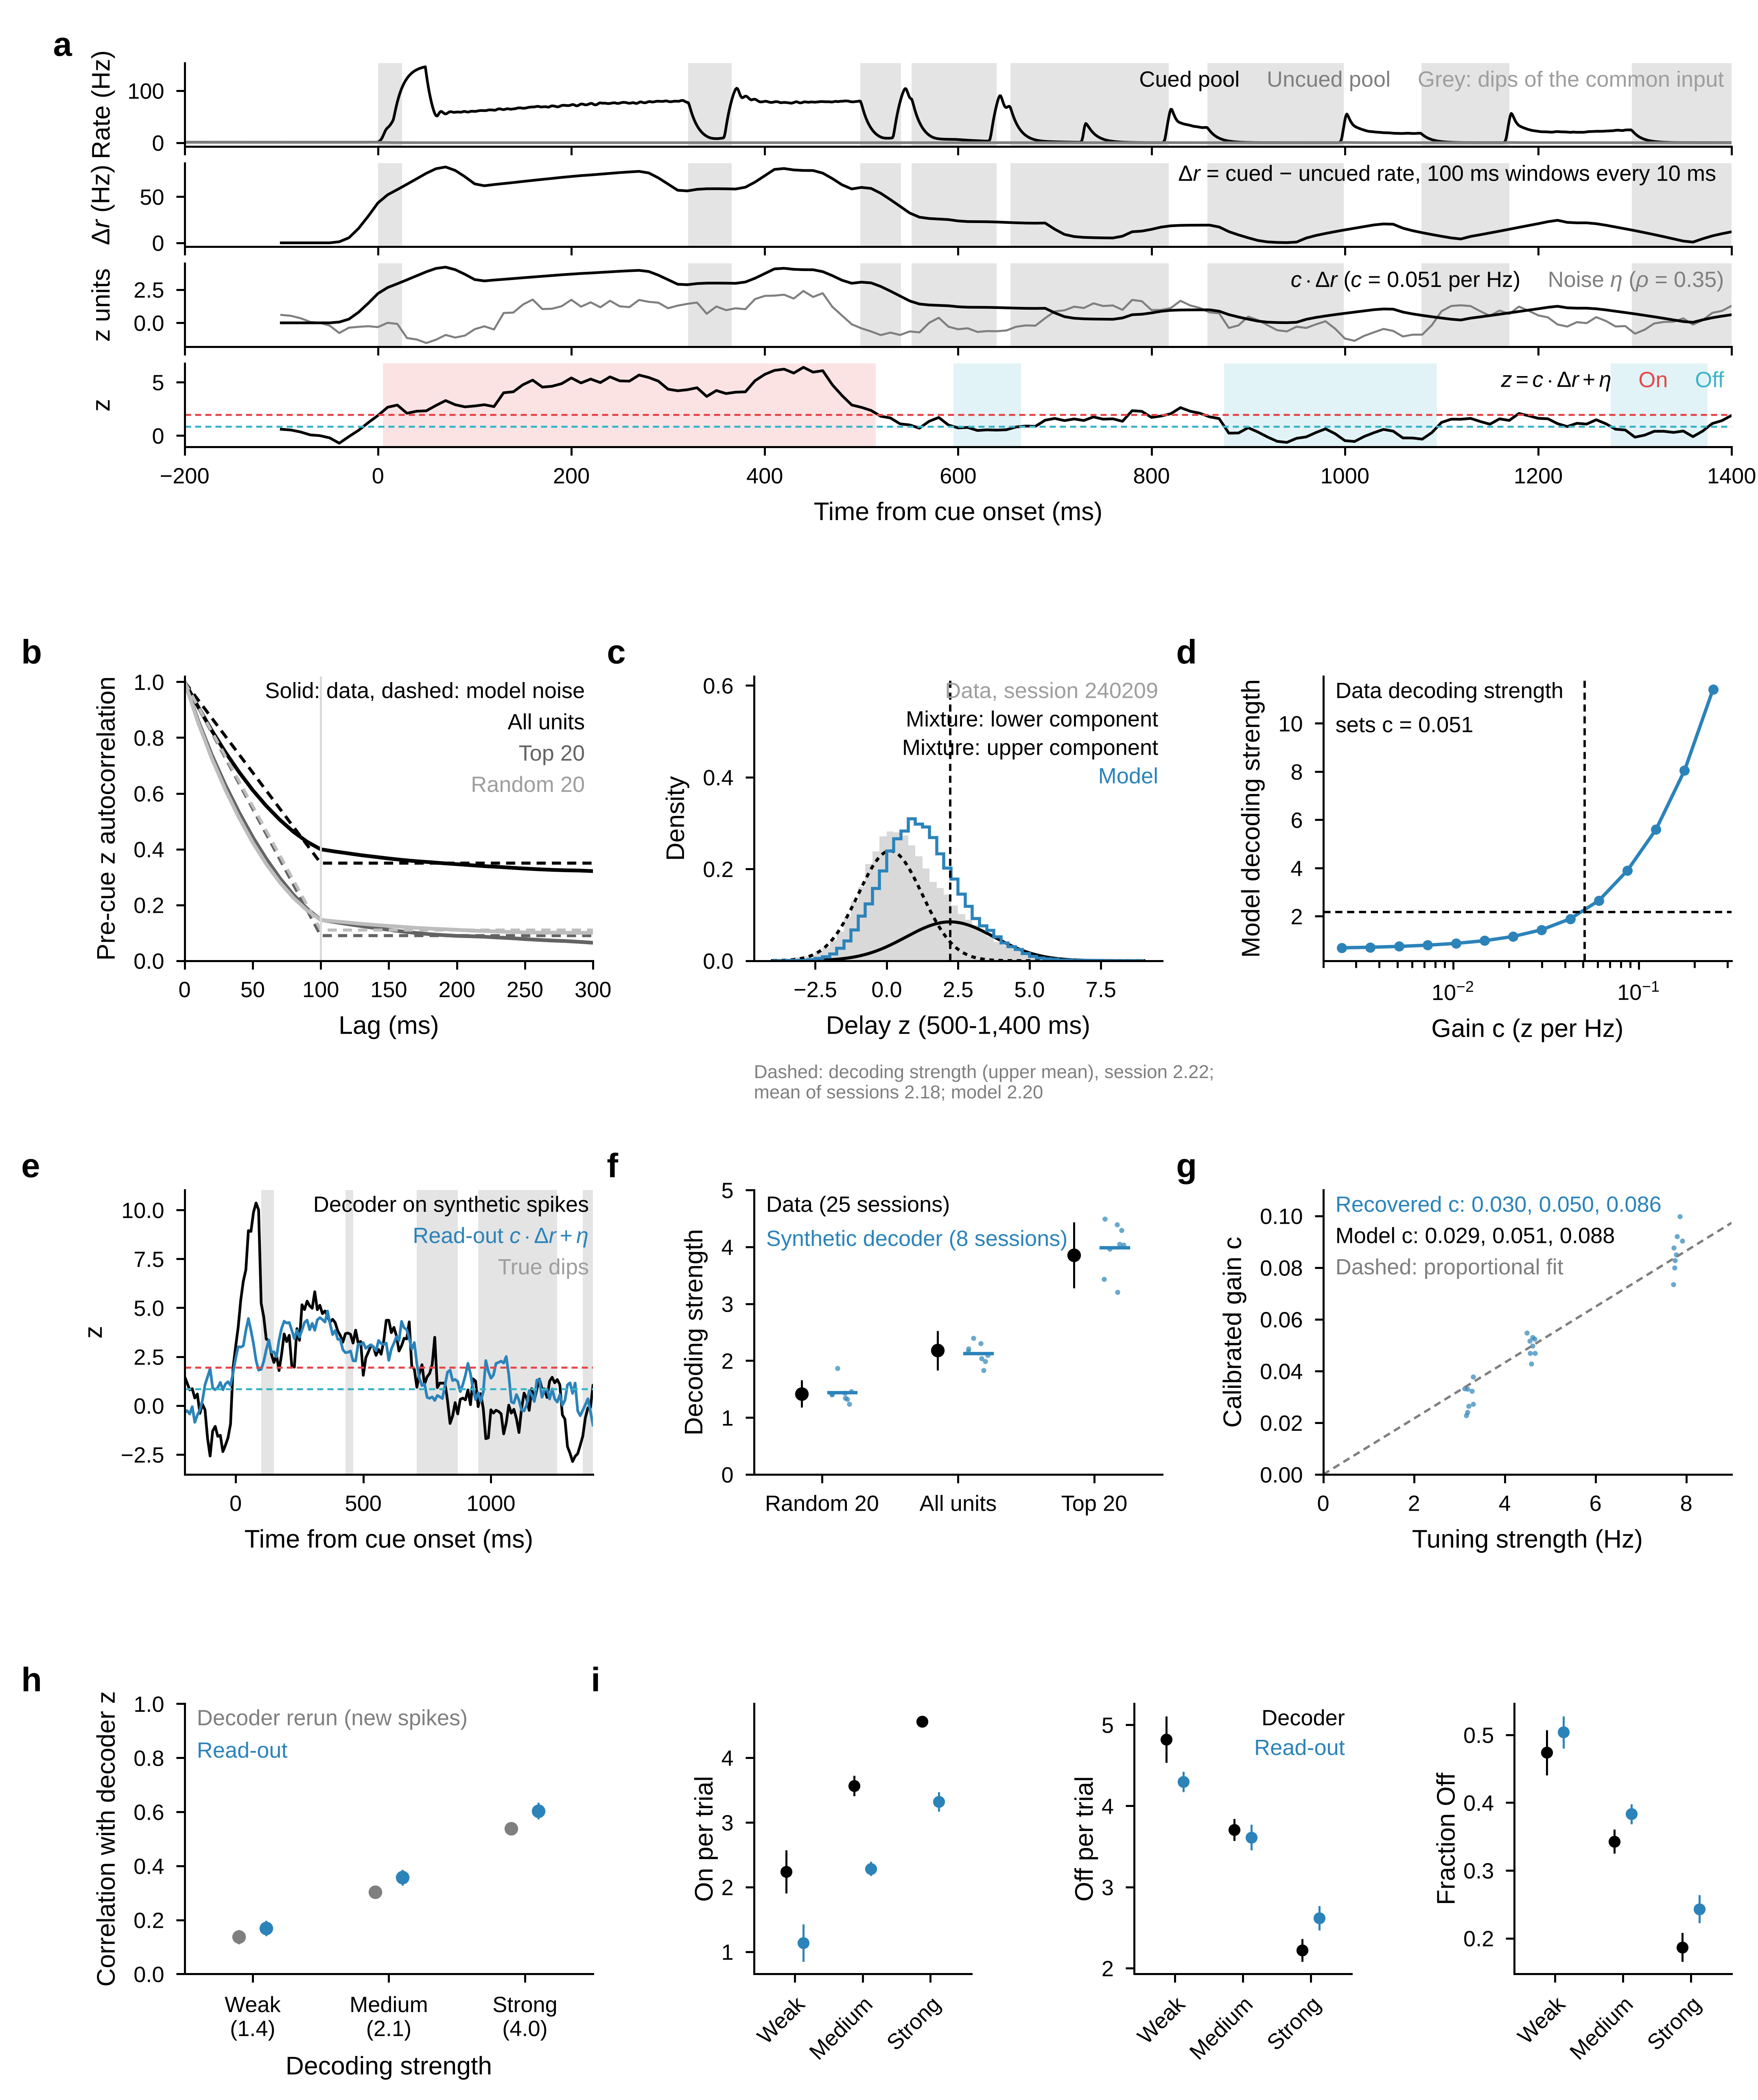
\includegraphics[width=0.923\textwidth]{figures/fig05.png}\end{center}

Supplementary Figure 1. Reading the model out like the data. a, One model trial through the read-out. From top to bottom, rates of the cued (black) and uncued (grey) pools, with dips of the common input in grey; \ensuremath{\Delta}r, their difference averaged in 100 ms windows every 10 ms; c\ensuremath{\cdot}\ensuremath{\Delta}r (black) and the read-out noise \ensuremath{\eta} (grey); and z = c\ensuremath{\cdot}\ensuremath{\Delta}r + \ensuremath{\eta}, with \textit{On} (red) and \textit{Off} (cyan) states labelled with the thresholds of Panichello et al. (2024) (dashed, z = 1.96 and 0.84). b, Autocorrelation of the decoder z before the cue, where there is no memory signal, for three decoded populations (solid; black, all units; dark grey, top 20; light grey, random 20), and of the model's noise \ensuremath{\eta} with the \ensuremath{\rho} of each population (dashed). The vertical line marks the 100 ms window, beyond which the correlation reflects the per-trial offset. c, Delay z (500–1,400 ms after cue onset) of one example session (grey; session 240209, whose decoding strength is closest to the mean over sessions), with the two components of a Gaussian mixture fitted to it (dotted, lower; solid, upper), and the model's delay z (blue). Dashed, decoding strength, the mean of the upper component (2.22 for this session, 2.18 averaged over sessions, 2.20 for the model). d, Decoding strength of the model as a function of the gain c. The data's decoding strength (horizontal line) sets c (vertical line). e–i, Validation on synthetic data. The fitted model drove 330 Poisson neurons, at three tuning strengths, and their spikes were decoded with the data pipeline. e, Example trial with the true dips (grey), the decoder's z (black) and the read-out z = c\ensuremath{\cdot}\ensuremath{\Delta}r + \ensuremath{\eta} (blue). f, Decoding strength of the synthetic decoder (blue, 8 sessions per tuning strength) and of the data's random-20, all-unit and top-20 decoders (black, mean \ensuremath{\pm} 2 SEM over 25 sessions). g, Gain c recovered by applying the data calibration to the synthetic decoder, against the tuning strength of the synthetic neurons. Dashed, proportional fit. h, Correlation of the read-out's delay z with the decoder's (blue), and of a rerun of the decoder on new spikes (grey), which sets the ceiling for two noisy read-outs. i, \textit{On} and \textit{Off} statistics of the decoder (black) and of the read-out (blue). h, i, mean \ensuremath{\pm} 2 SEM over 8 synthetic sessions.

\begin{center}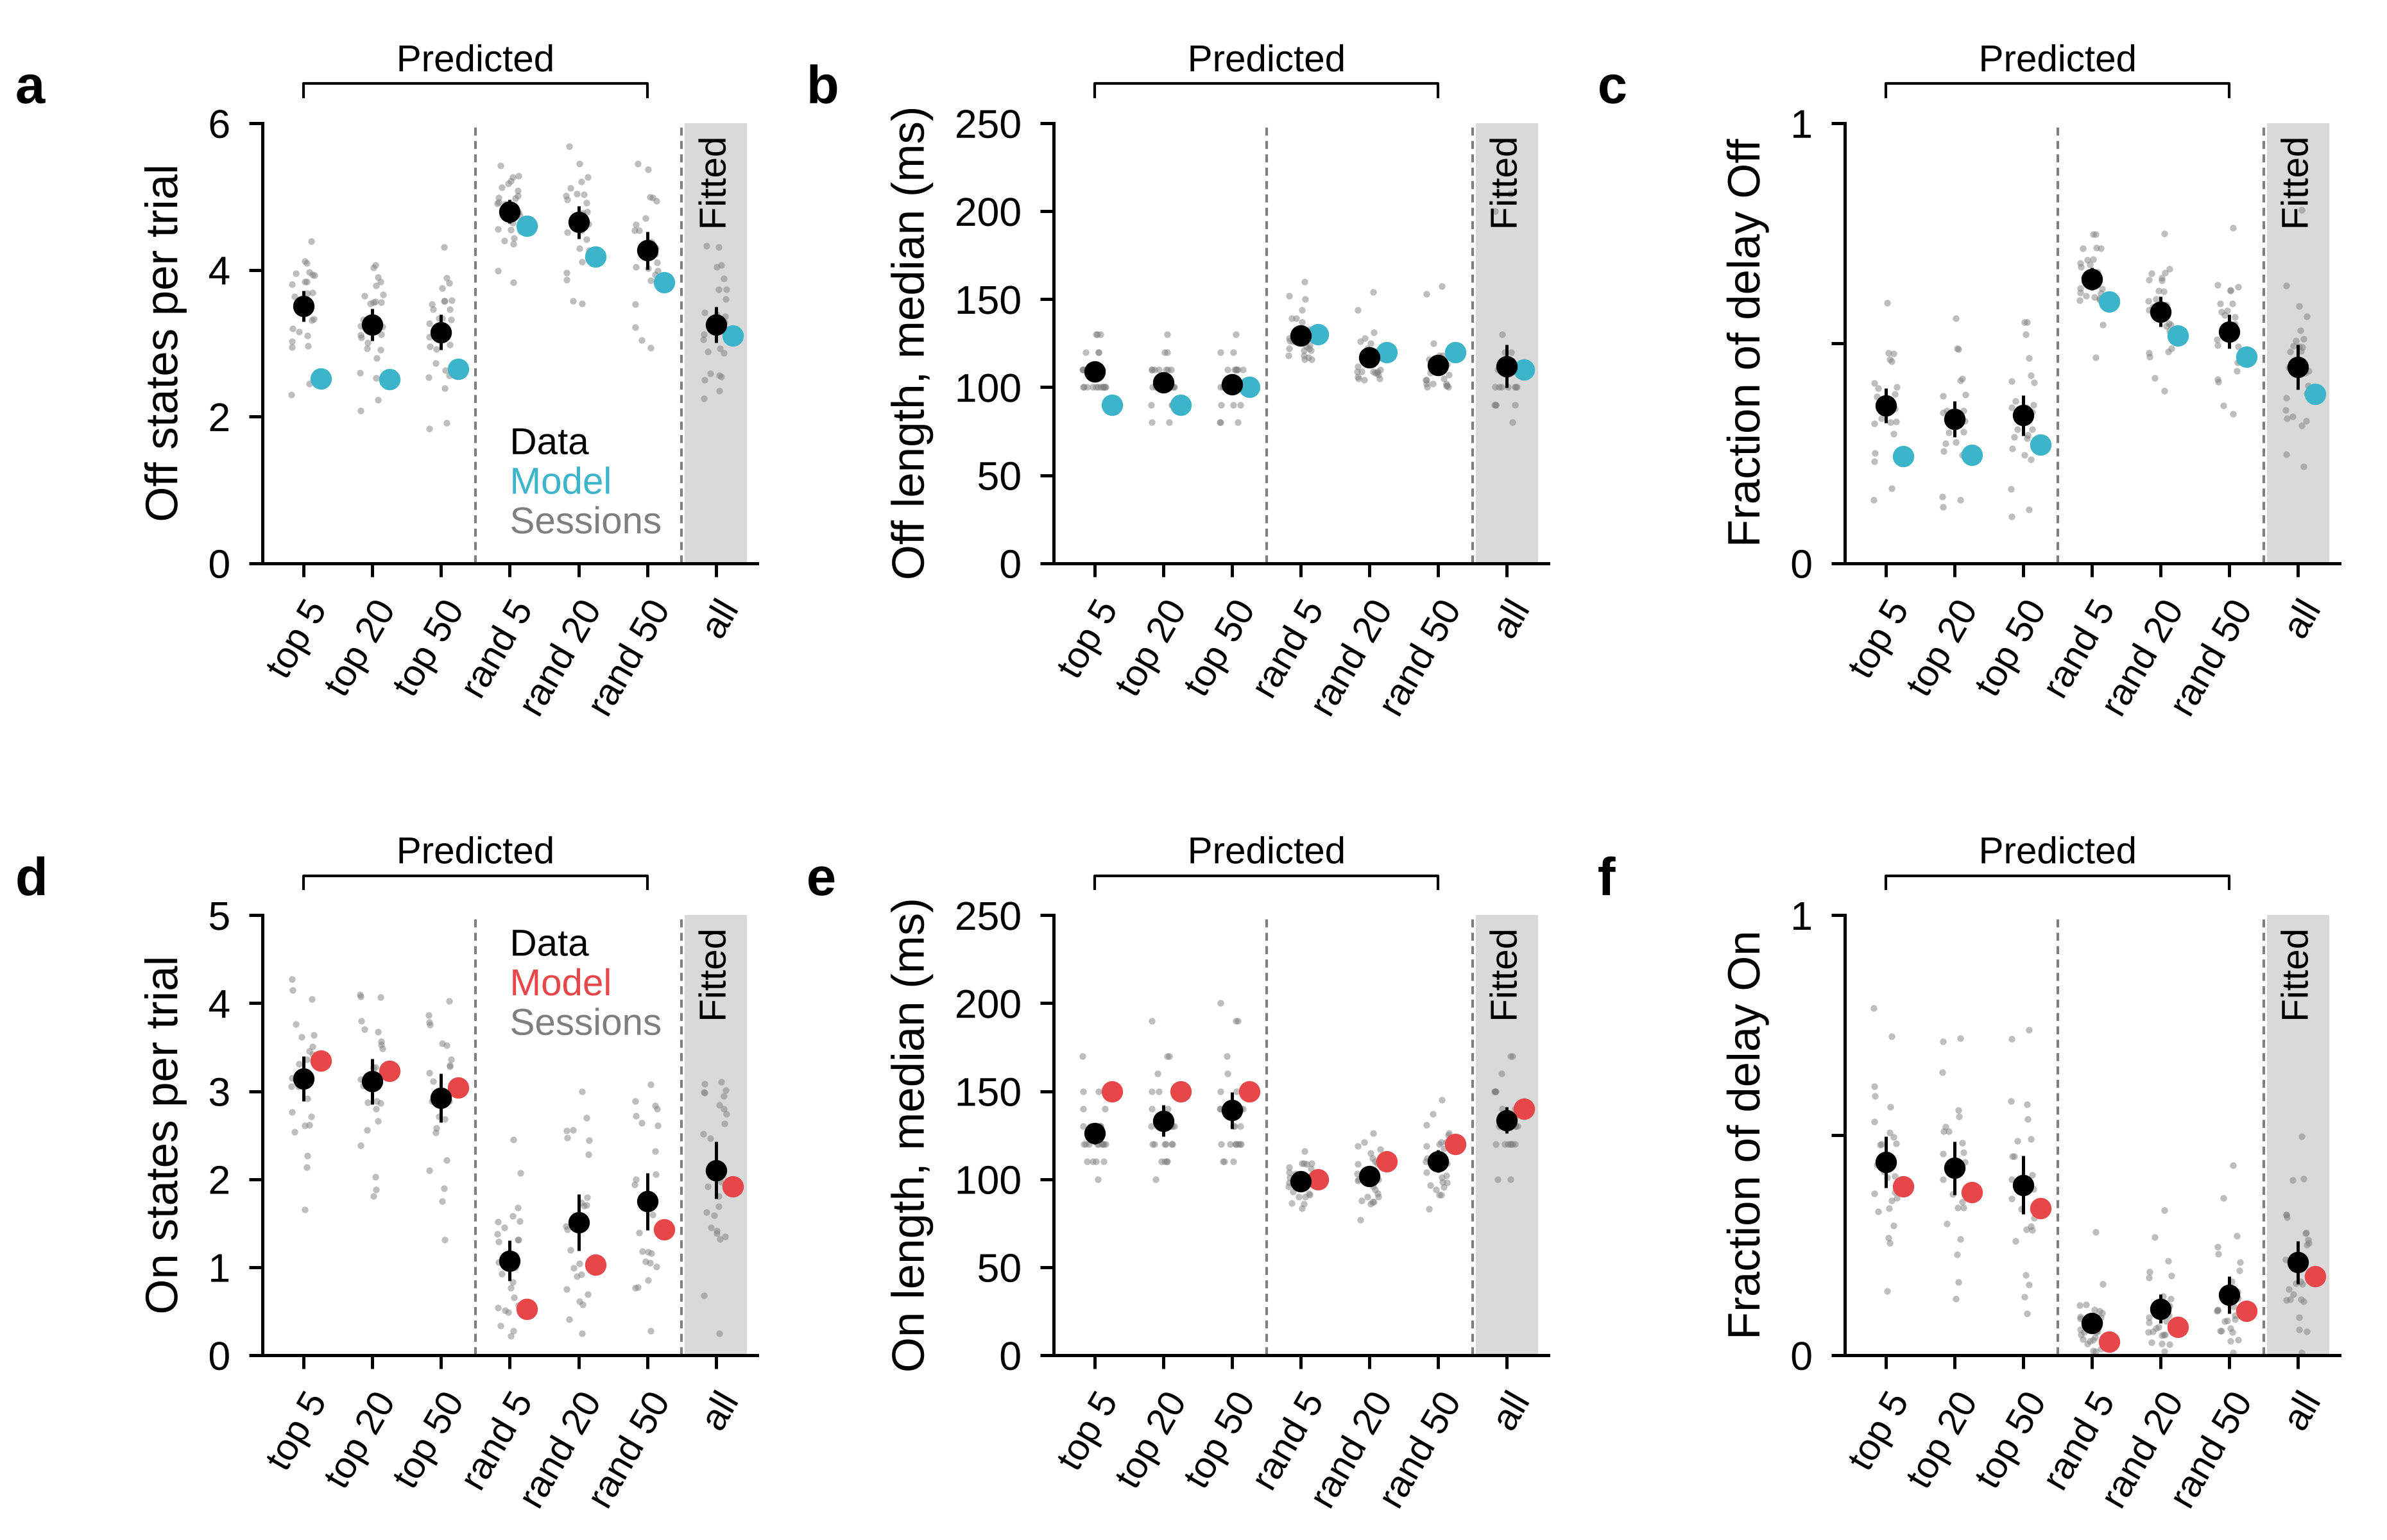
\includegraphics[width=0.923\textwidth]{figures/fig06.png}\end{center}

\textbf{Supplementary Figure 2. }\textbf{\textit{On/Off}}\textbf{ statistics of each decoded population, data and model.} Decoders using the most cue-selective neurons (top 5, 20, 50) are \textit{On} more often and \textit{Off} less often than decoders using the same numbers of random neurons (rand 5, 20, 50). Black circles: data, mean \ensuremath{\pm} 95\% CI (2 SEM) over 25 sessions. Grey dots: single sessions. Cyan and red circles: model, \textit{Off} and \textit{On} statistics. The model was fitted to all neurons only (grey band). The other six decoded populations are predictions obtained by changing only the read-out gain and noise (Methods).

\begin{center}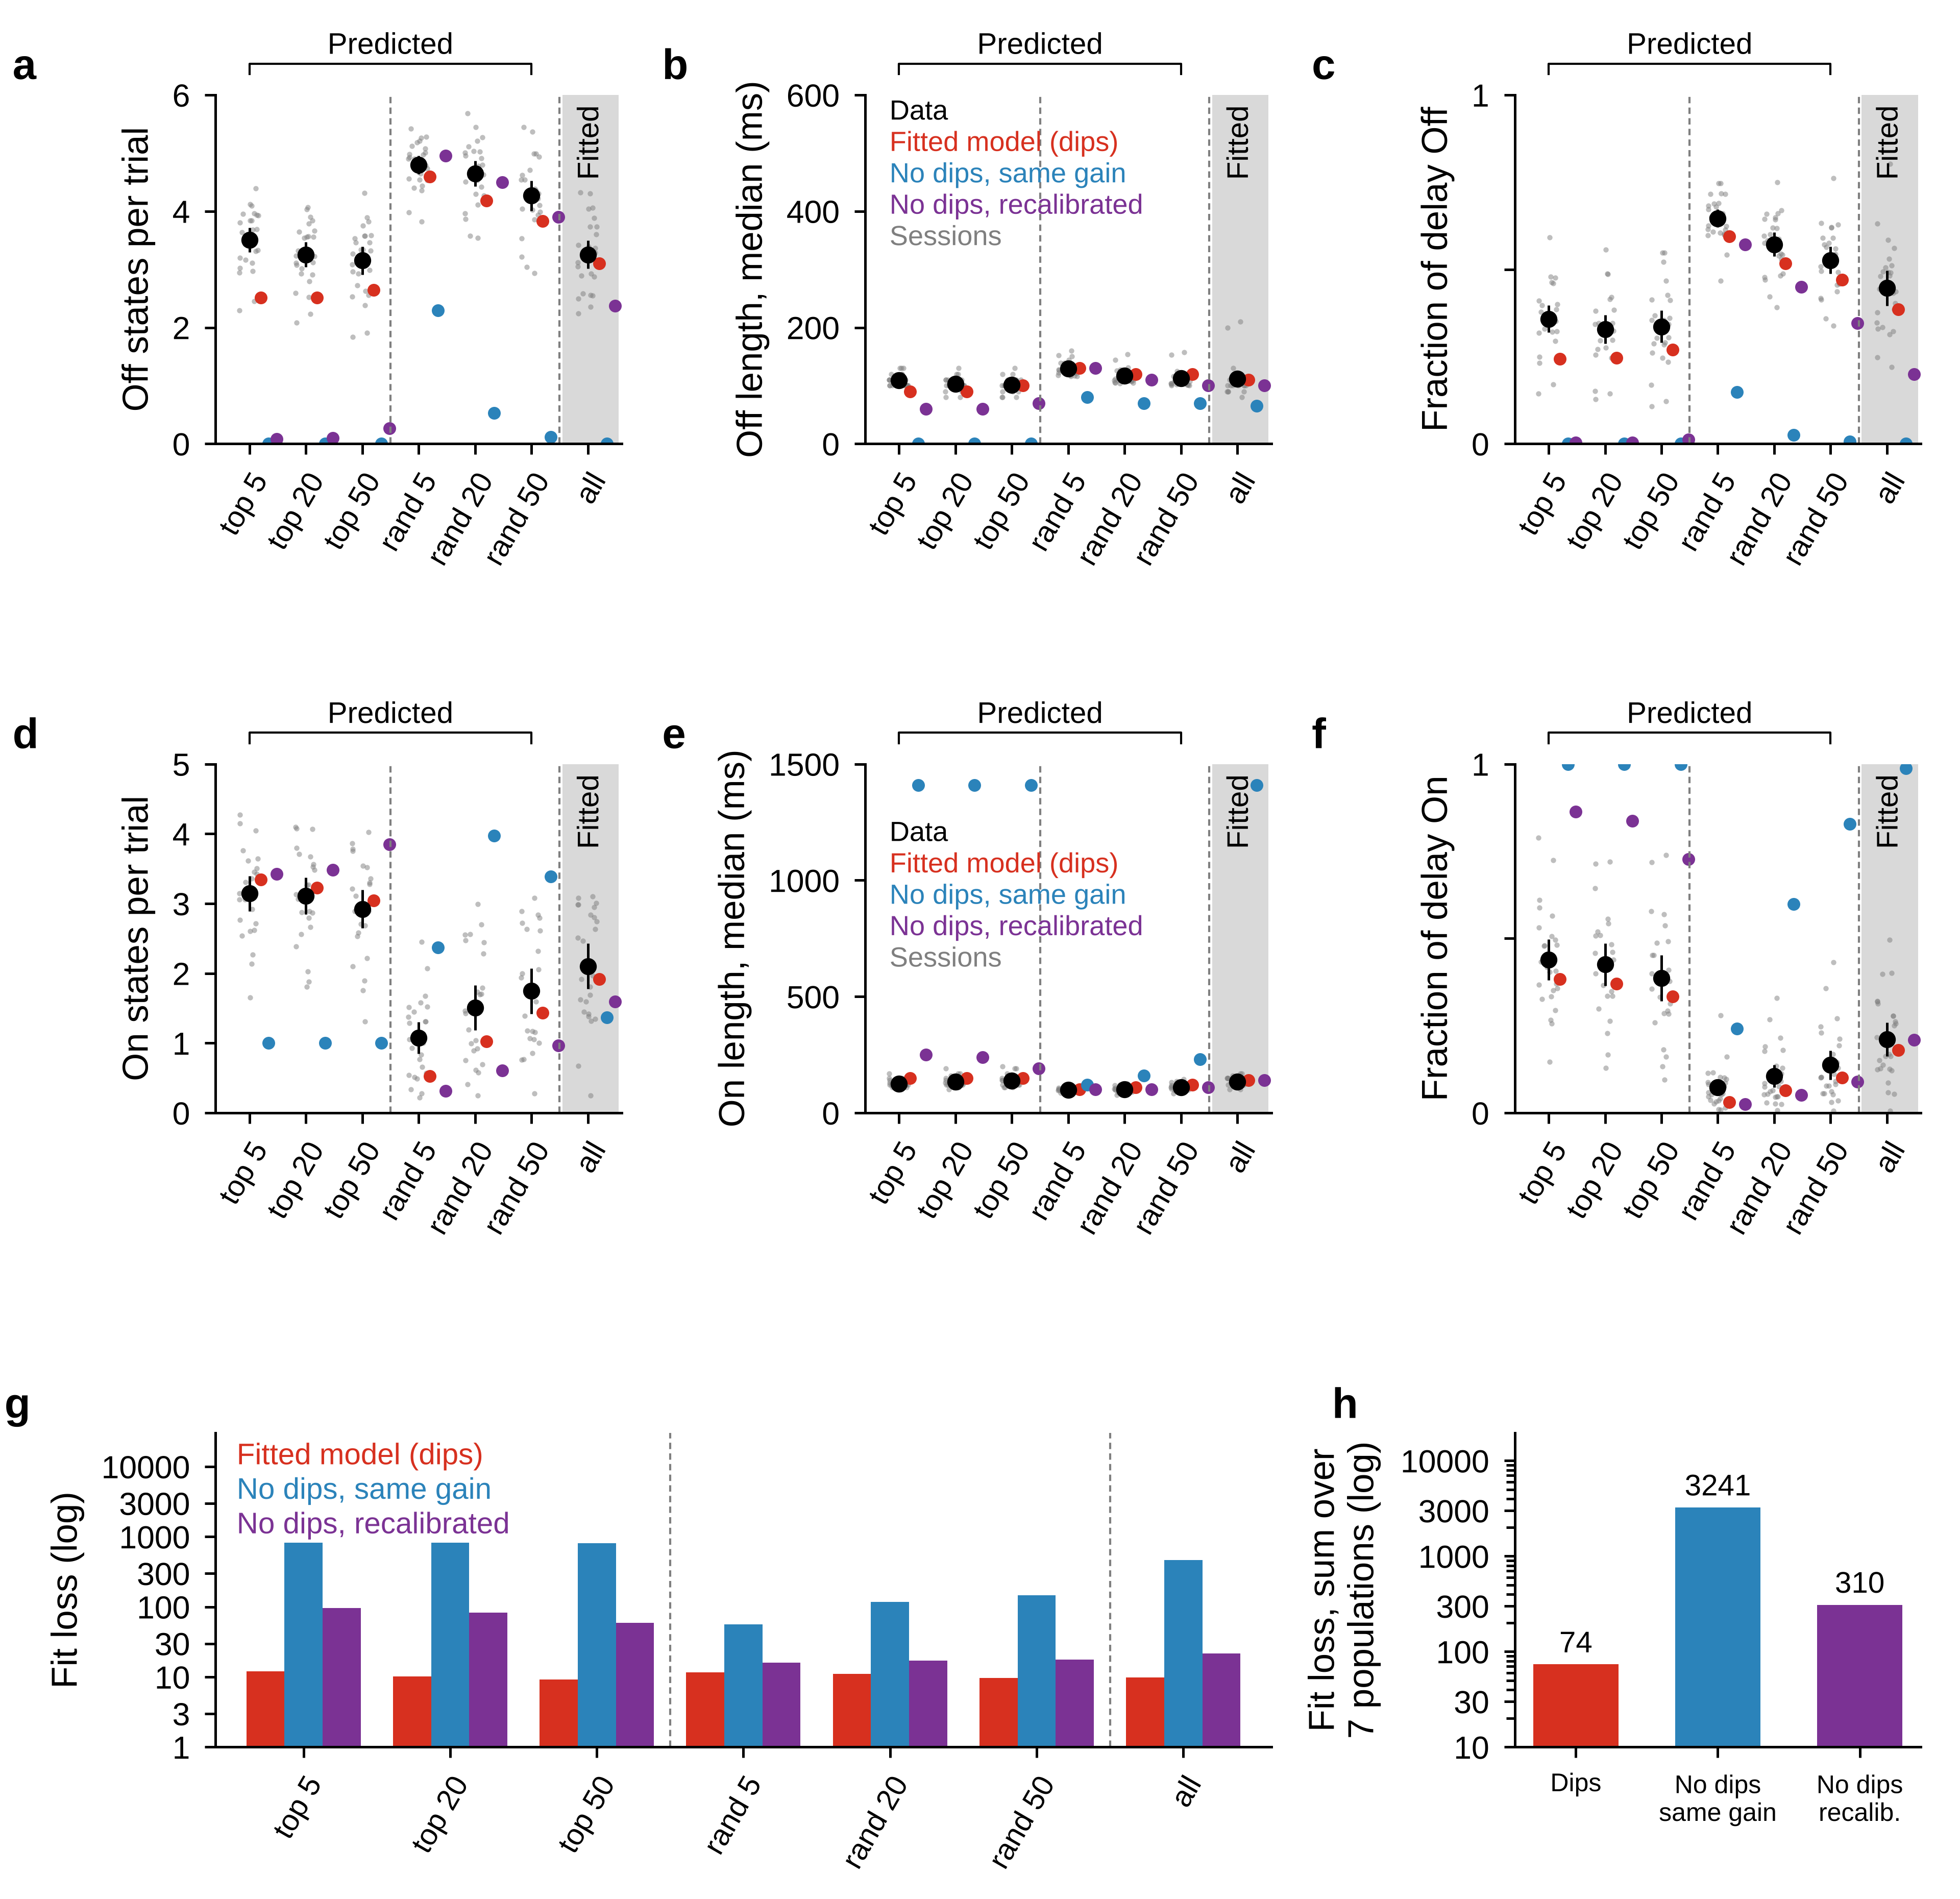
\includegraphics[width=0.923\textwidth]{figures/fig07.png}\end{center}

\textbf{Supplementary Figure 3. }\textbf{\textit{Off states}}\textbf{ are not produced by the read-out noise alone.} \textit{On/Off} statistics of the seven decoded populations, as in Supplementary Fig. 2: a, \textit{Off states} per trial; b, median \textit{Off} length; c, fraction of the delay \textit{Off}; d, \textit{On states} per trial; e, median \textit{On} length; f, fraction of the delay \textit{On}. Black circles, data (mean \ensuremath{\pm} 2 SEM over 25 sessions). Grey dots, single sessions. Red, fitted model (with dips). Blue, the same model with a constant common input (no dips), read out with the identical read-out (same gain, noise and labelling) for each population. Purple, the no-dip model with the read-out gain recalibrated to each population's decoding strength in the data. Without dips, the identical read-out produced no \textit{Off states} for the top-unit and all-unit decoders and fewer than the data for random neurons (0.1–2.1 vs 4.3–4.8 per trial). With the gain recalibrated, noise alone reproduced the \textit{Off states} of the random populations but not those of the top-unit decoders (0.1–0.3 vs 3.2–3.5 \textit{Off states} per trial), and for all units it gave 2.4 per trial, against 3.3 in the data and 3.1 in the fitted model (summed fit loss over the seven populations 310, vs 74 for the fitted model). g, Fit loss of each condition for each decoded population (the loss used for fitting, Methods; log scale). h, Fit loss summed over the seven decoded populations.

\begin{center}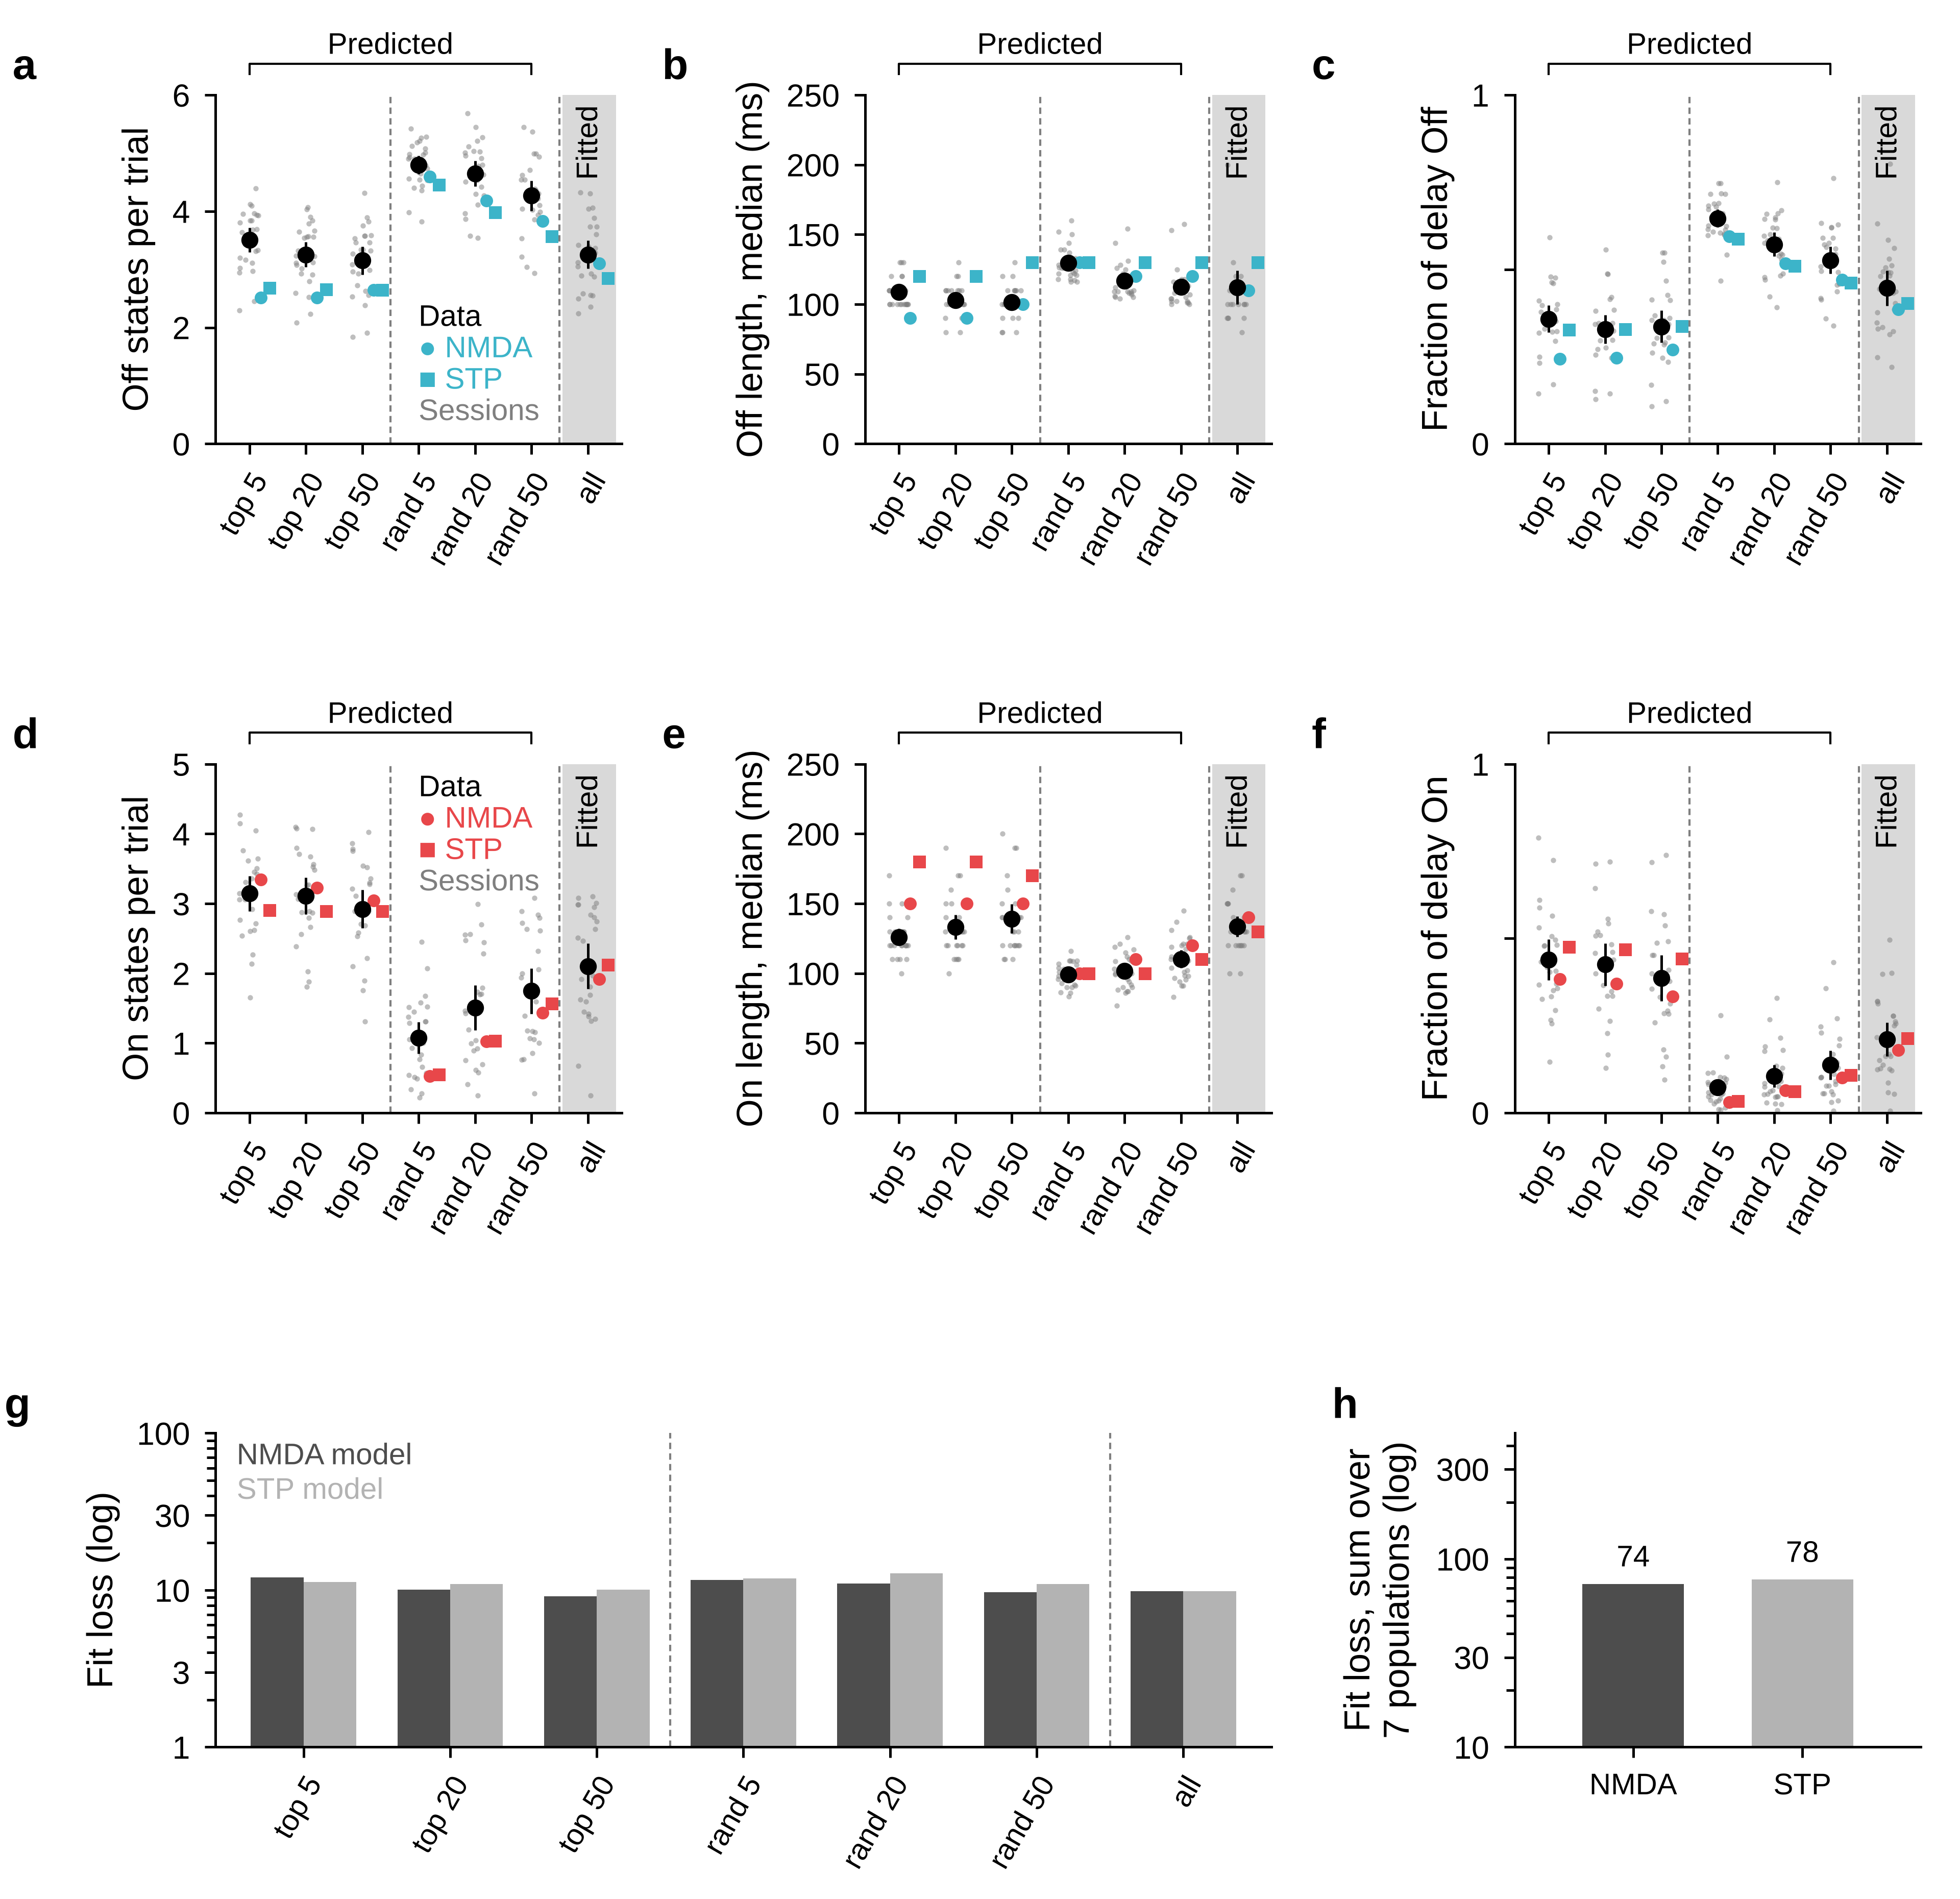
\includegraphics[width=0.923\textwidth]{figures/fig08.png}\end{center}

Supplementary Figure 4. The STP model fits the \textit{On/Off} statistics about as well as the NMDA model. As Supplementary Fig. 2, for the NMDA model (circles) and the STP model, in which short-term facilitation replaces NMDA gating (squares; Methods). Both models were fitted to the decoder using all neurons only (grey band), and the other six decoded populations are predictions obtained by changing only the read-out gain and noise. Black circles, data (mean \ensuremath{\pm} 2 SEM over 25 sessions). Grey dots, single sessions. Cyan and red symbols, model \textit{Off and On} statistics. g, Fit loss of each model for each decoded population (the loss used for fitting, Methods; log scale). h, Fit loss summed over the seven decoded populations.

\end{document}
